\documentclass[defaultstyle,11pt]{thesis}

\usepackage{amssymb}		% to get all AMS symbols
\usepackage{amsmath}		% to get equations to work right
\usepackage{graphicx}		% to insert figures
\graphicspath{{../}{Trap/}}
\usepackage[pagebackref = true]{hyperref}		% PDF hyperreferences?? [backref=none]
\usepackage{natbib}
\usepackage{array}
\newcolumntype{L}[1]{>{\raggedright\let\newline\\\arraybackslash\hspace{0pt}}m{#1}}
\newcolumntype{C}[1]{>{\centering\let\newline\\\arraybackslash\hspace{0pt}}m{#1}}
\newcolumntype{R}[1]{>{\raggedleft\let\newline\\\arraybackslash\hspace{0pt}}m{#1}}
\usepackage{caption}
\setcitestyle{numbers,square,comma}
\usepackage[usenames,dvipsnames]{color}
%% To make \href colors more decent:
\definecolor{MyDarkBlue}{rgb}{0,0.1,0.7}
\hypersetup{pdfborder={0 0 0},colorlinks,breaklinks=true,
  urlcolor={MyDarkBlue},citecolor={MyDarkBlue},linkcolor={MyDarkBlue}
}
\renewcommand{\thefootnote}{\alph{footnote}}	
\title{a}
\abstract{a}
\author{a}{a}
\otherdegrees{a}
\degree{a}{a}
\dept{a}{a}
\advisor{a}{a}
\reader{a}
\readerThree{a}
\SuspendPrologue
\begin{document}
\input macros.tex

\chapter{Molecular Trapping}

Some of the earliest successful trapping of neutral molecules began with CaH in John Doyle's group in a dilution fridge with $^3$He buffer~\cite{Weinstein1998}.
Stark decelerated and electrostatic trapped ammonia followed soon later~\cite{Bethlem2000trap}.
Since then extensions to many species have occurred. 
In this chapter we focus on OH molecules, whose strong Stark shift to mass ratios make them favorable for attempts to attain high enough densities to observe collisions between members of the ensemble.

%% SECTION HISTORY OF OH TRAPS
%% SECTION HISTORY OF OH TRAPS
\section{History of OH traps}

%Trap History Table
\renewcommand{\arraystretch}{1.5}
\begin{table}[t!]
\centering
\caption{
The Ye Group Molecule trapping endeavor.\label{trappingtable}
}
\label{tab:rates}
\begin{tabular}{ L{2.5cm} | C{4.5cm} C{2.5cm} C{4.5cm} }
Name & Type & Depth (mK) & Uses \\
\hline\hline
MET 	& Magnetic Quadrupole, Electric Hexapole & 250 	& First Demonstration~\cite{Sawyer2007} 	 \\
\hline
Ring 		& Magnetic Quadrupole				& 100 	& He, D$_2$, ND$_3$ Collisions~\cite{Sawyer2008,Sawyer2011} \\
\hline
Ring 		& Above, but new mounts				& 100 	& E-field Induced Collisions,  Evaporation~\cite{Stuhl2012uwave,Stuhl2012evap,Stuhl2013} \\
\hline
Tricycle 	& Magnetic Quadrupole 				& 300 	& 10x density, spin-flip loss \\
\hline
Pin  		& 2D Magnetic and Electric Quadrupoles 	& 500 	& Solved spin-flip loss~\cite{Reens2017}\\
\hline
Cryocycle 	& Magnetic Quadupole 				& 200 	& Lifetime, Fluorescence Enhancements\\
\end{tabular}
\end{table}

The history of OH trapping in the Ye group has grown substantial enough to warrant a tabular environment~\ref{trappingtable}. 
Each attempt has brought new challenges and experiences, and steady progress has been made in a number of key areas.
The Magnetoelectrostatic Trap (MET) installed during Brian Sawyer's time~\cite{Sawyer2007} was a heroic first attempt that included a few-turn magnetic coil run at a startling $1400$~A, and $2000$~A briefly during loading.
Later it was decided to trade the role of the fields used for loading, and great gains in magnetic field strength and simplicity were attained by switching to permanent magnets with the ``Ring'' trap~\cite{Sawyer2011}.
A key improvement occurred when it was discovered that patch charges on the Ultem mounts originally used for affixing the magnetic trap to the Stark decelerator could have a significant impact on spectroscopic efforts~\citep[Fig.~6]{Stuhl2012uwave}.
This was addressed by designing primarily stainless steel mounts, so that molecules only had line of sight to grounded conductors, although still with insulators installed between the decelerator and trap but relocated elsewhere.

% SECTION TRICYCLE OVER RING TRAP
% SECTION TRICYCLE OVER RING TRAP
\section{Tricycle over Ring Trap}

In pursuit of increases in density and molecule number, an iteration on the Ring trap was performed, dubbed the ``Tricycle'' trap due to the three rectangles formed when examining planar cuts through the ring and rear magnets used to generate the trap, see Fig.~\ref{ringtricyclefigure}.
This was first installed in 2014, and improved on the Ring trap in several key ways:
\begin{enumerate}
\item Replaced rear ring with its core, removing an outer toroidal trap and tripling depth.
\item Significantly improved loading dynamics.
\item Increased trap gradient, thanks to a $\sim 40\%$ reduction in size.
\end{enumerate}

\begin{figure}[t!]
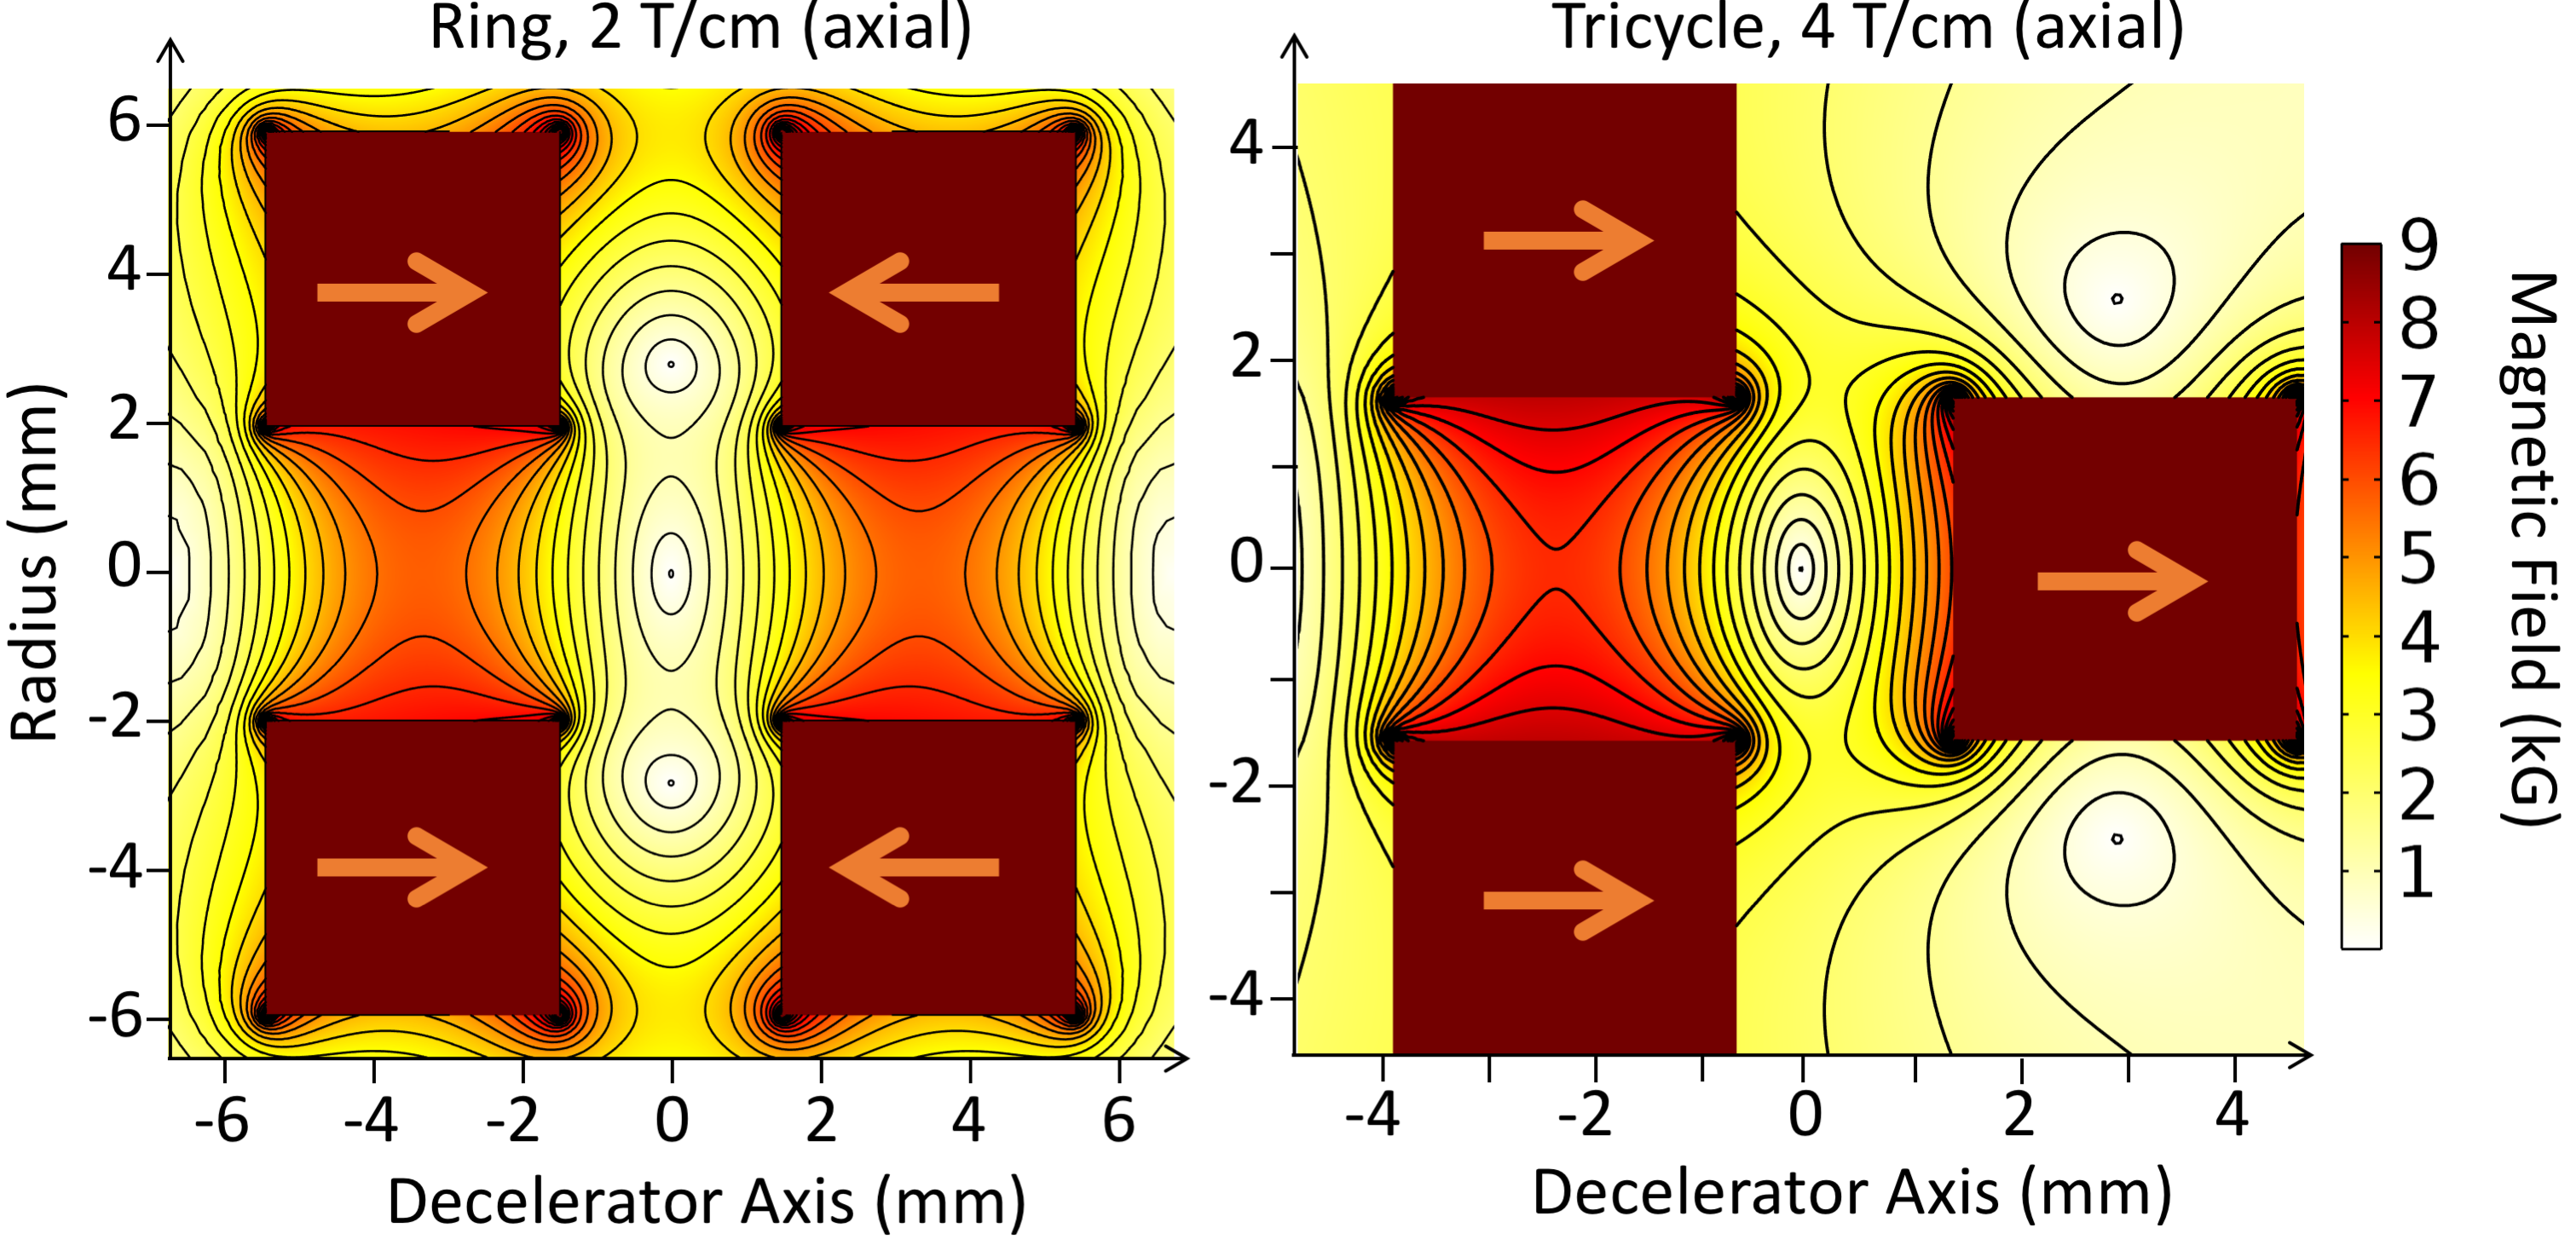
\includegraphics[width=\linewidth]{RingTricycle.png}
\caption[Ring and Tricycle Trap Comparison]{\label{ringtricyclefigure}
Cross Sections including the cylindrically symmetric axis for both the Ring and Tricycle traps. Arrows indicate magnetization directions up to an overall sign. Magnetic trapping fields are shown, demonstrating the destabilization of the toroidal minimum of the Ring trap. Contours every $500$~G. Steel mounting electrodes are not shown in either case, but are installed on the outer diameter of the magnets and affixed to them with setscrews.
}
\end{figure}

%SUBSECTION TOROIDAL DESTABILIZATION
\subsection{Toroidal Destabilization}

This first achievement was one of the primary goals of the iteration, since the influence of the toroidal minimum present in the Ring trap was difficult to ascertain. 
Molecules ought to have been able to explore the toroidal region, but based on the observed distribution of molecules as a function of magnetic field, they did not appear to be doing so for unknown reasons.
At the time it was highly desirable to be able to perform the same evaporation type experiments, but in a geometry without a toroidal minimum.
The removal of the toroidal minimum can be best understood by thinking about the traps using the principle of superposition.
The Ring trap may be thought of as the result of superposing two different quadrupole traps, one formed by cylinders of diameter given by the ID of the rings, and the other formed by cylindrical magnets of diameter given by the OD of the rings.
The smaller quadrupole trap is nice and tight, but the magnets block the beam path.
The larger trap is larger and weaker, and its field lines move in the opposite direction, since its magnets are oppositely magnetized relative to the smaller quadrupole trap (so that they cancel each other out in the centers of the rings, allowing molecules to pass through).
The larger trap works against the smaller, but is much weaker than it at least near the center of the geometry, so that the smaller remains somewhat tight near the trap center.
Further outside, where the fields generated by the smaller quadrupole trap are less significant, the outer quadrupole dominates, creating the outer toroidal minimum.
If instead of overlapping a larger quadrupole trap with the smaller, we just overlap a single disk magnet, then no significant outer trap is created, just as in the Tricycle trap.

In fact, in the limit of large OD of the single ring magnet of the Tricycle trap, the geometry exactly approaches that of a pair of small disk magnets, but with the crucial modification of an entry hole for the molecules to be delivered.
This is because for a disk magnet, the on-axis magnetic field is given by:
\begin{equation}
B(z) = \frac{1}{2}B_r\left(\frac{z+t}{\sqrt{R^2+(z+t)^2}} - \frac{z-t}{\sqrt{R^2+(z-t)^2}}    \right),
\end{equation}
where $B_r$ is the remanent flux density of the permanent magnet, $t$ is its half thickness, and $z$ the distance from the magnet center, and $R$ gives the cylinder radius. In the limit of large $R$ we obtain:
\begin{equation}
B(z) = \frac{1}{2}B_r\left( \frac{z+t}{R+(z+t)^2/2R)}  - \frac{z-t}{R+(z-t)^2/2R)}   \right),
\end{equation}
and taking it to cubic order:
\begin{eqnarray}
B(z) &=& \frac{1}{2}B_r\left( \frac{z+t}{R} - \frac{(z+t)^3}{2R^3}  - \frac{z-t}{R} + \frac{(z-t)^3}{2R^3}   \right)\\
&=& \frac{1}{2}B_r\left(\frac{2t}{R} - \frac{3z^2t}{R^3} + \frac{t^3}{R^3} \right).
\end{eqnarray} 
So we see that as $R$ grows, $B(z)$ shrinks close to the magnet with $1/R$, but the flatness of the field increases, so that the term proportional to $z^2t/R^3$ which describes the second order fall off of the field away from the magnet reduces as $1/R^3$.
In other words, the magnetic field just outside of a disk magnet does indeed shrink as one increases its radius, although the volume occupied by this smaller magnetic field increases.
It is especially advantageous to have a small field from the large superimposed disk of the tricycle trap, since this extra field acts to shift the trap center into the hole of the ring and out of view of the detection laser.
For this purpose, the Tricycle trap features a $19$~mm outer diameter ring magnet, up from $12$~mm in the Ring trap.

%SUBSECTION LOADING IMPROVEMENTS
\subsection{Loading Improvements}

The Tricycle trap features very significant loading improvements over the Ring trap, although the precise extent is difficult to pin down. 
The main reason for an expectation of improvement lies in the phase space dynamical behavior of the two geometries.
In analyzing any trap loading scenario, it is important to pursue the analysis with both intuition and simulation.
The latter on its own will lack the guidance necessary for truly identifying an optimal scenario, while the former is unlikely to be able to fully disentangle interdependent factors influencing performance.

On the intuitive side, it is useful to use the same reasoning as in the decelerator by focusing on phase stability.
The loading fields generated by charging up the surfaces of the ring magnets in the Ring trap are mirror symmetric about the center of the Ring trap.
This means that if a loading sequence is designed so that the synchronous molecule ends up exactly in the trap center, the synchronous molecule will be required to roll up to the top of a hill and then stop there. 
Molecules with slightly more forwards velocity than the synchronous molecules will end up quite a ways down the other side of the hill by the time the loading fields are switched off, and vice versa.
In layman's terms, longitudinal phase stability during loading requires that the loading be performed on a slope, not a peak.

It is possible to generalize these ideas further, while still remaining in the intuitive domain.
If it is true that the loading fields ought to feature a slope at the location of the trap center where the synchronous molecule comes to rest, what is the ideal value for that slope?
Also, is there a similar ideal value for the slope of the loading fields in the region in front of and beyond the trap center?
We can answer these questions with a simplified thought experiment, refer to Fig.~\ref{LoadingRotation}.
Suppose we have a population experiencing a harmonic trapping potential with a characteristic width $\delta z$ in real space and $\delta v$ in velocity space, and centered at $z_0=0$ and $v_0 > 0$.
One way to controllably transfer this population to $v_0=0$ without unwanted stretching of the population would be to load it into a much larger harmonic potential with oscillation frequency $\omega$ centered at $z=0$ and $v=0$.
Because harmonic potentials always execute rotations in phase space with ellipticity controlled by their oscillation frequency, the population would then be smoothly transferred over the course of a quarter oscillation to be centered at $z = v_0/\omega$ and $v=0$, with widths $\omega\delta z$ and $\delta v/\omega$.
If $\omega$ is chosen equal to $\delta v/\delta z$, i.e. to have the same strength as the trapping potential prior the initiation of the loading sequence, then the original widths in position and velocity are precisely maintained.
On the other hand, $\omega$ could be tuned so as to optimize coupling between the initial traveling trapping potential and the trapping potential to be used after loading.

\begin{figure}[t!]
\centering
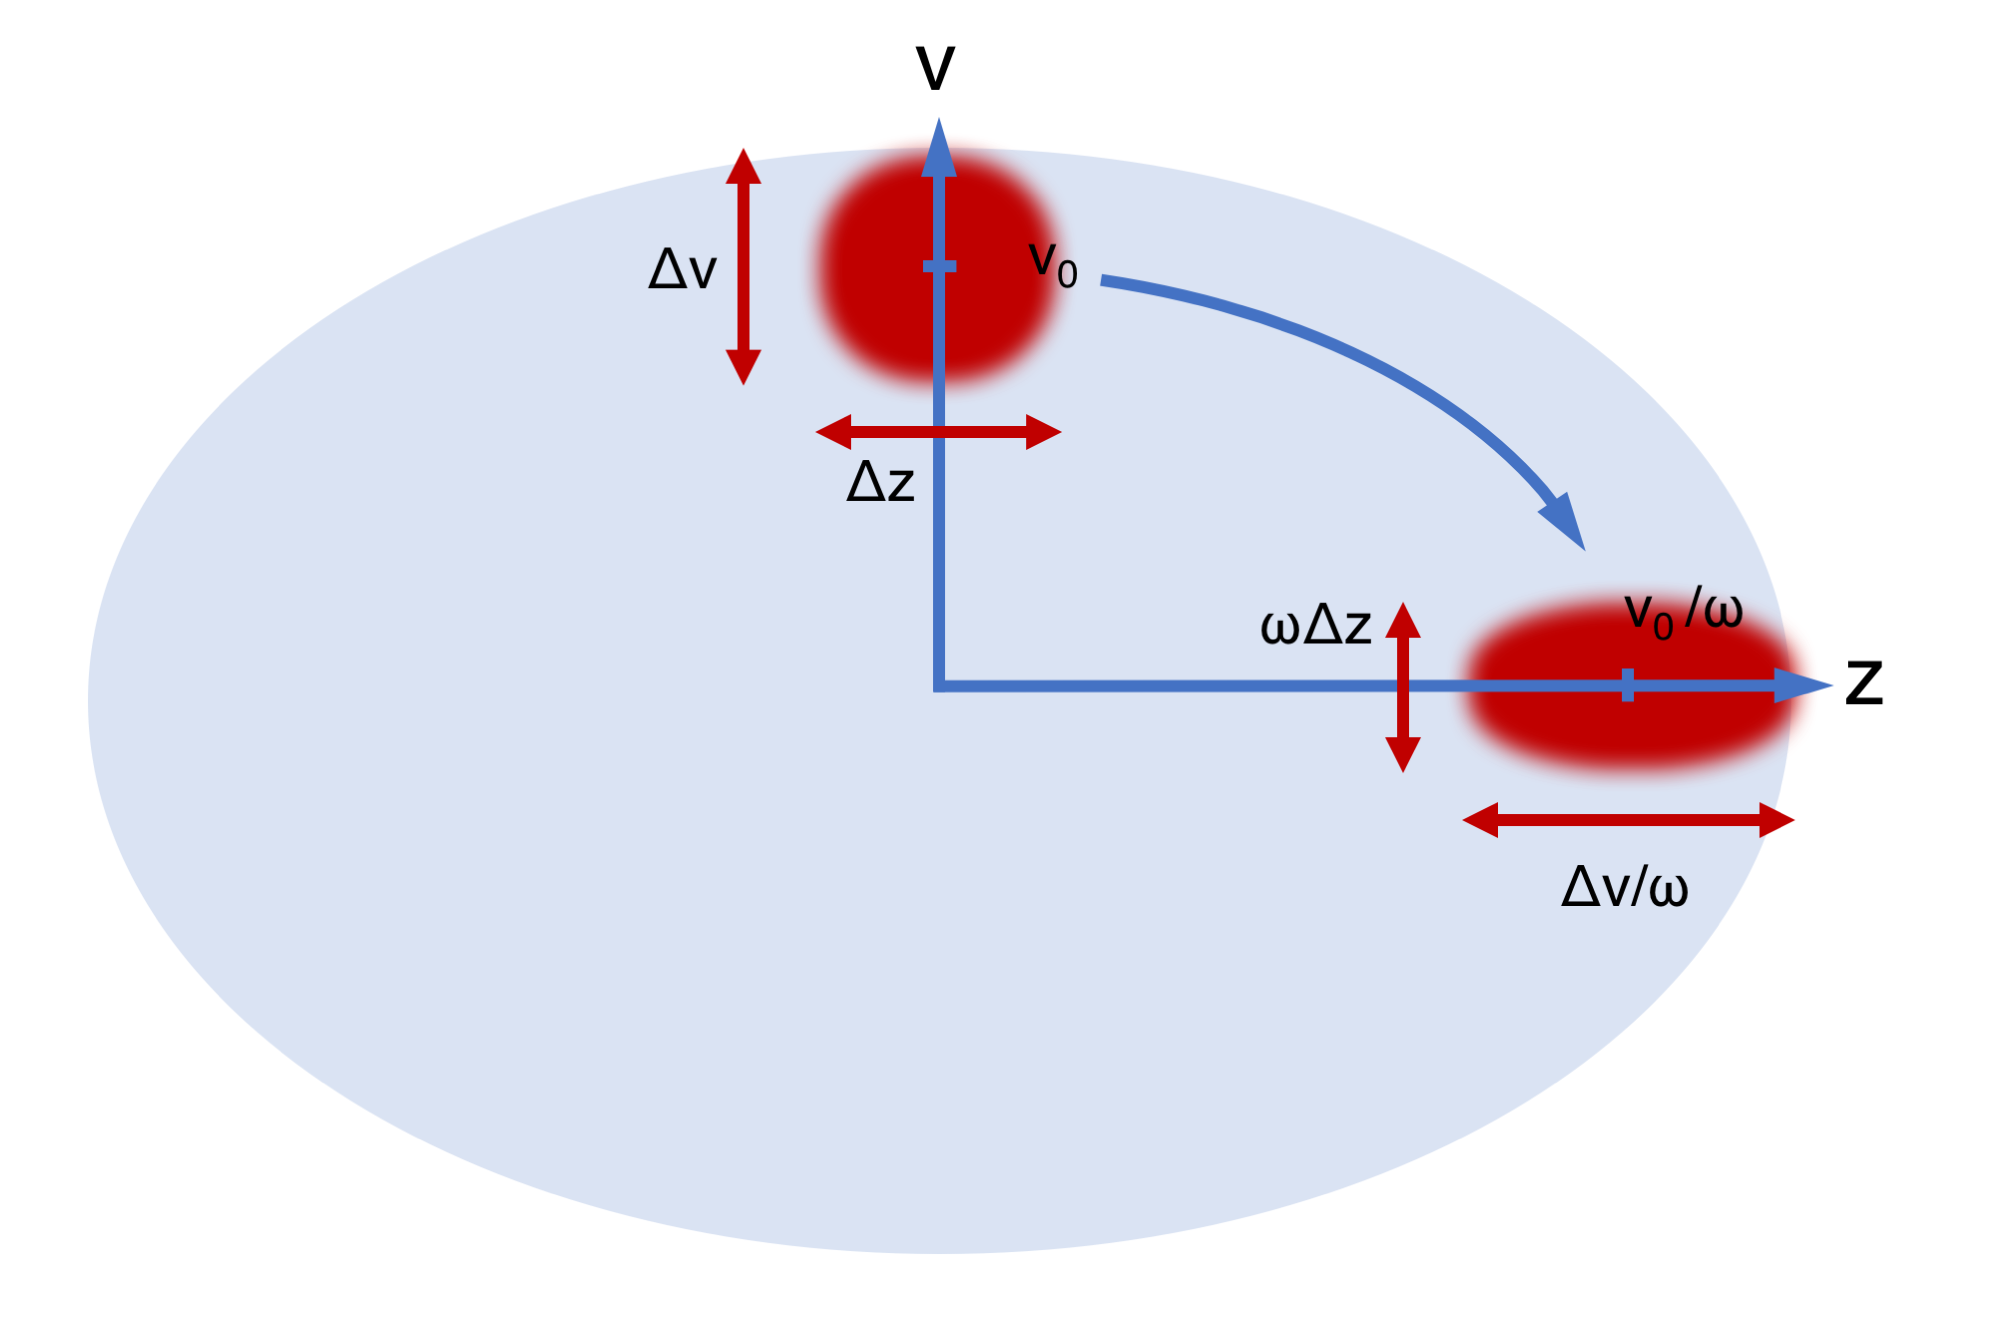
\includegraphics[width=10cm]{LoadingRotation.png}
\caption[Ideal Trap Loading as a Quarter Rotation]{\label{LoadingRotation}
Phase space diagram depicting the action of the ideal phase space conservative loading fields derived from a large external harmonic potential. The region of phase space acted on by the external potential is indicated as a light blue ellipse. The region of phase space populated initially is shown in red along the $v$ axis. The region populated after rotation is shown along the $z$ axis also in red. Widths and origins are as indicated.
}
\end{figure}

In addition to this harmonic loading potential, it would be ideal to also maintain a transverse trap simultaneously. 
The ideal fields would have a magnitude with the following spatial dependence:
\begin{equation}
|E(x,y,z)| = \frac{1}{2}m_{OH}\left(\omega_z^2z^2 + \omega_r^2r^2\right)
\end{equation}
where $\omega_z$ and $\omega_r$ are the longitudinal and transverse trap frequencies.
Neglecting the nonlinearity of the Stark shift for OH molecules close to zero field, such a harmonic potential could be generated transversely with a hexapole, but to do it simultaneously in the transverse and longitudinal directions would require an octupole moment, such as could be generated with three rings and two endcaps with the endcaps at $+V$, the outer rings grounded, and the inner one at $-V/2$ so as to approximate spherical boundary conditions following the second Legendre polynomial~\cite{jackson1999classical}.
This would of course be very unlikely to be able to be crammed into the small space between the end of a decelerator and a trap, and unlikely to be able to be charged up to a high enough potential energy for stopping an appreciable speed $v$.
It is much more likely that an efficient solution would be obtained by abandoning the harmonicity and instead focusing on the reduced criterion of loading fields that respect phase stability by having a slope at the location of what will be come the trap center and which also provide some transverse confinement.
The slope of the loading field at the location of the trap center would ideally match the slope that the ideal harmonic trap with frequency $\omega$ would have at that point, $m_\text{OH}\omega v_0$.

\begin{figure}[t!]
\centering
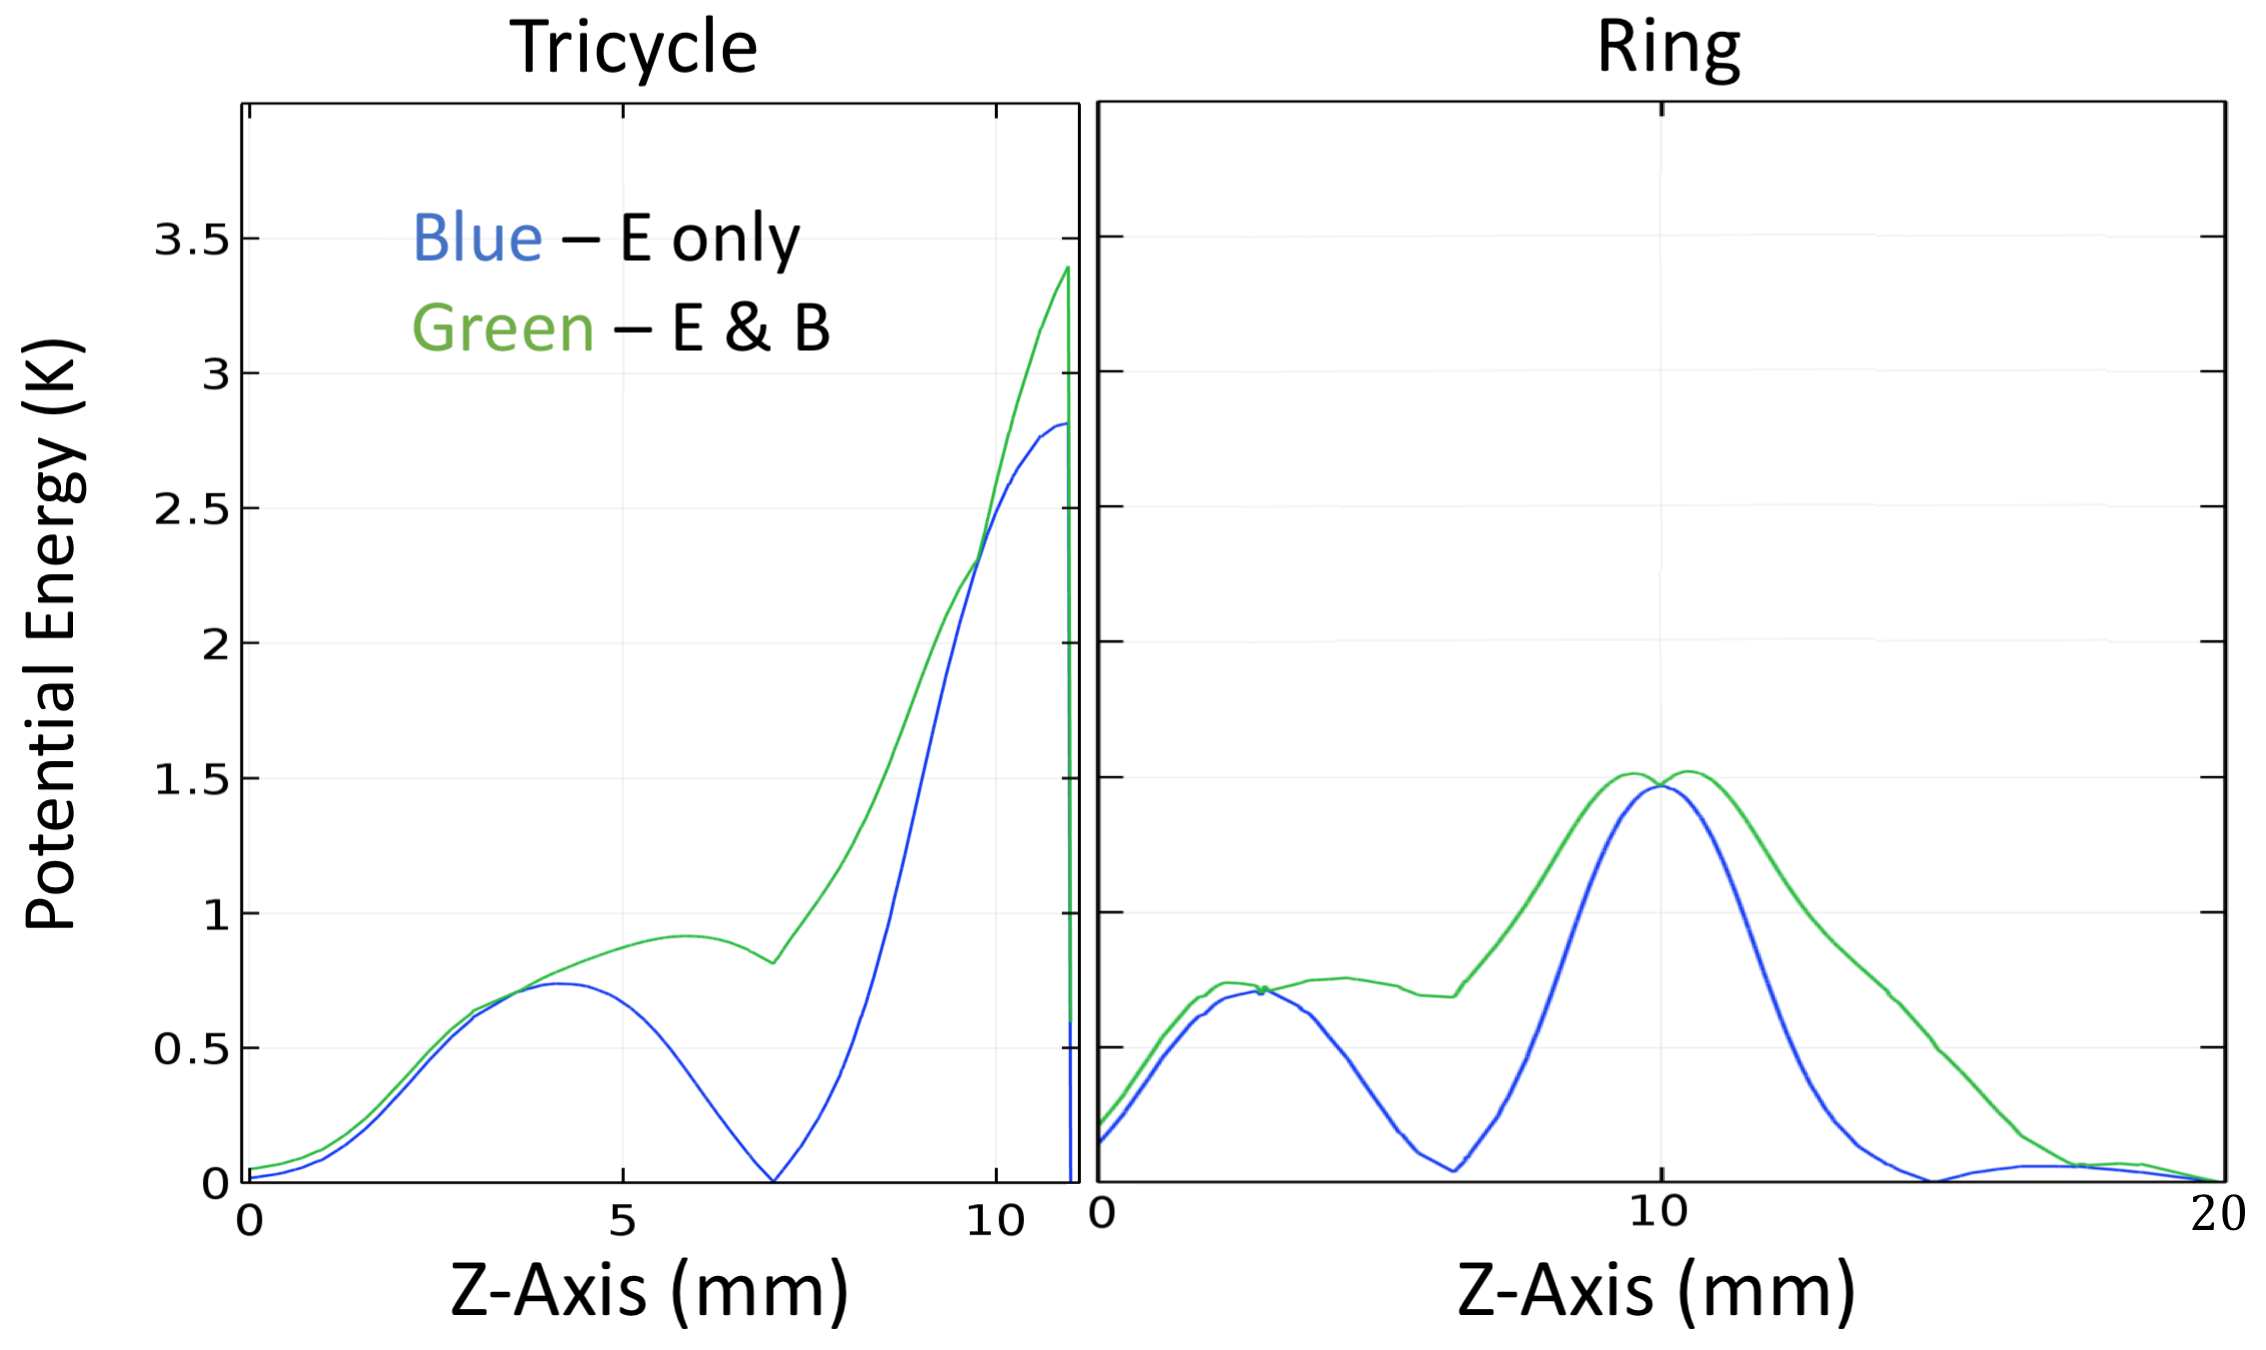
\includegraphics[width=14cm]{LoadingFieldsEB.png}
\caption[On-Axis Loading for Ring and Tricycle]{\label{loadingringtrike}
Potential energy along axis for Ring and Tricycle traps. The trap center is located at $z=10$~mm in both cases. Note the more favorable slope of the loading potential in the vicinity of the trap center for the tricycle trap. Field magnitudes arise from application of $\pm12.5\text{ kV}$ for the Ring trap and also for the Tricycle. In practice almost half this voltage was applied on the Tricycle for optimal operation, perhaps due to arcing effects or nonadiabatic transitions during loading discussed below in Sec.~\ref{loadingtransitions}.
}
\end{figure}

In practice, Fig.~\ref{loadingringtrike} shows what we are able to obtain for loading fields comparing the Ring and Tricycle traps.
Note the role of the magnetic field, which is non-negligible.
The tricycle trap comes much closer to the harmonic ideal discussed above.
For the ring trap, the extra effect of the magnetic field actually depresses the potential energy at the trap center below a wider plateau, making it formally impossible to bring the synchronous molecule to rest at the trap center.
In practice, the experimentally determined ideal application time of loading fields likely corresponds to the synchronous molecule being brought close to rest but out in front of the trap center.
This unideal situation should result in a higher loaded temperature in the ring trap compared with the tricycle trap, $87$~mK compared with $61$~mK in simulation.
In practice however, the measured spectra of molecules in the Ring trap fits better to a thermal distribution and to a lower temperature compared with the tricycle trap, see Fig.~\ref{RingTriSpectrum.png}.
Before discussing this further, we first revisit the process of spectroscopy in these traps.

% SUBSECTION MICROWAVE SPECTROSCOPY
\subsection{Microwave Spectroscopy}

A critical tool for understanding the behavior of populations in our magnetic traps is microwave spectroscopy performed on the parity changing transition between \f3 and \e3 states.
This transition is ideal for spectroscopy, because it has a very small but nonetheless nonzero differential Zeeman shift of $26.6$~MHz/T, which allows molecules to be resolved according to their magnetic field, while also allowing the entire trap to be surveyed over a very narrow bandwidth of microwave frequencies.
The narrowness of the band is crucial for avoiding the complexities associated with the delivery of microwaves to the trapping region.
If it were necessary to instead use microwaves to transfer molecules directly from a trapped to an untrapped state by flipping their magnetic quantum number, \f3 to \fm3, scanning the trap would require scanning the applied microwave frequency between $1.7$ and $16$~GHz.
While this is no problem for the microwave synthesizer itself, obtaining a suitably level passband in the components responsible for delivering the microwaves to the molecules would be unfeasible.
In particular, the microwaves are delivered to the trap using a bias tee setup, nicely described in~\citep[Fig.~5]{Stuhl2012uwave}, and the transfer function through the isolation capacitors is particularly troublesome, see Fig.~\ref{broadercoupling.png}.
In contrast, with the entire population sitting below $0.5$~T, only $13$~MHz needs to be scanned out of $1.7$~GHz, and no significant attenuation variation is expected or measured.

\figdave{broadercoupling.png}{Microwave Coupling through Bias Tee}{Microwave transfer function from vacuum feedthrough to magnet surfaces. Large variations are observed across the GHz scale required for performing spectroscopy along $m$-changing transitions, but not on the MHz scale required for \f3 to \e3 spectroscopy.}{10cm}

In addition to the use of microwaves to transfer population, the spectroscopy relies on a few further steps.
First, molecules in the \e3 state remain trapped, and must be removed.
This is done by first applying a bias electric field to allow molecules to escape via avoided crossings, as discussed in Chapter~\ref{chapter:Background}.
In~\cite{Stuhl2012uwave}, it was nicely demonstrated that this is effective for removing molecules in the $|e\rangle$ state.
Second, the process is repeated many times, with varying wait times so as to avoid any pathological resonance between the application of microwaves and the oscillation of molecules in the trap, which could result in certain privileged classes of molecule orbits always avoiding the microwaves.
Third, comparison is made between the total laser induced fluorescence with and without the application of the spectroscopic sequence.
When this is done, spectra such as shown in Fig.~\ref{RingTriSpectrum.png} are obtained.

\figdave{RingTriSpectrum.png}{Spectra in Ring and Tricycle Trap}{Spectra in the Ring and Tricycle traps after loading with no evaporation. The former was published in \citep[Fig.~3a]{Stuhl2012evap}, the latter was collected on Feb.~24, 2014.}{\linewidth}

% SUBSECTION LIMITATIONS TO SPECTROSCOPY
\subsection{Limitations to Spectroscopy}\label{limitationsection}

One key limitation to microwave spectroscopy via the procedure described is the spatial variation of sensitivity of the technique.
The influence on microwave frequency dependent intensity has already been claimed negligible, but microwave intensity at any given frequency varies significantly across the cloud.
This goes against the rule of thumb that electromagnetic intensity shouldn't vary significantly on lengthscales below a wavelength, $18$~cm in this case.
This is because the microwaves are in the near field regime with respect to the conductors that form the trapping potential.
The microwave fields may to a good approximation be taken to be dominantly electric and equal to the DC electric field distribution generated during loading but with magnitude oscillating at the microwave frequency.
This means that their intensity should vary as shown in Fig.~\ref{NearFieldUWave.png}ab.
In particular, the microwave intensity falls off quickly as molecules approach the openings of the magnets of the Ring trap.
Furthermore, the efficiency of microwave transfer also features a polarization dependence.
Since the \f3 to \e3 transition has $\Delta m=0$, there is a dependence of the Rabi frequency describing the intensity of the microwave drive on the cosine of the angle $\theta$ between the electric and magnetic fields, see panel~(c) of Fig.~\ref{NearFieldUWave.png}.
This ends up favoring molecules on the axis of the trap.

\figdave{NearFieldUWave.png}{Near Field Microwave Intensity in Ring and Tricycle Trap}{The near field intensity close to the (a) Tricycle trap and (b) Ring trap. Colors and contours are relative to the magnitude of the microwave drive, but may be thought of as ranging from $0$ to $100\%$ as color ranges from black to red to yellow to white, with contours at $5\%$ intervals. Colors are comparable between the two traps, assuming the same microwave intensity on the surface of the conductors. These are also the DC field distributions for loading the traps, in which case color ranges from $0$ to $200$~kV/cm with contours every $10$~kV/cm and $25$~kV applied across the magnet surfaces. Rings are $3$~mm apart for the Ring trap and in the Tricycle trap magnets are $2$~mm apart. (c) The angle between electric and magnetic fields is shown, from red, $0$, to blue, $\pi/2$ radians. Magnetic field contours every $500$~G are superposed.}{\linewidth}

In mid 2013, an effort was made to perform spectroscopy along the \f3 to \e1 transition, with the goal of addressing the issue that \e3-state molecules with total energies below the lowest crossing of the \e3 and \fm3 states at $410$~G are unable to find their way out of the trap, see Fig.~\ref{sigmaspec.png}.
The results were quite different from those performed along the \f3 to \e3 transition, perhaps due to polarization differences since this transition would feature dependence on $sin(\theta)$, but more likely reflective of the microwave coupling bandwidth issues discussed above.

\figdave{sigmaspec.png}{Spectroscopy from \f3 to \e1}{Depletion spectroscopy performed by microwave transfer from the \f3 to \e1 state. The dip between $800-1000$~G is likely an artifact of coupling efficiency challenges.}{10cm}

Another point is the spatial dependence of the fluorescence collection system.
Fig.~\ref{Collection.png} shows how the solid angle for photons to hit the lens varies with trap position, but beyond this there is of course the question of laser coverage.
The laser is always optimized for signal, making it quite likely to be well overlapped with the trap center, but for the larger magnetic field ranges, there are regions of the trap that are likely not well exposed to the laser, especially inside the rings of the traps, since the laser impinges from the side.

\figdave{Collection.png}{Ring and Tricycle Collection Solid Angle}{Collection solid angle for the Tricycle (left) and Ring (right) traps. Colors do not quite match between the two panels but are labeled in steradians. For the tricycle trap, the lens is located far below, while for the ring trap it is located far above. Electrodes are to the left and right of the plots. In both cases, solid angle variations within $500~\mu$m of the trap center are on the $10\%$ level only, although larger variations occur for molecules regularly reaching $3-5$~kG, a deviation of over $1$~mm from the trap center.}{16cm}

Some of these spatial variations may be mitigated by an ergodic hypothesis.
If the molecules can be assumed to be exploring all regions of phase space, then variations in detection efficiency may not significantly perturb the spectra or prevent it from representing the thermal state of the ensemble.
Essentially, any blind spots in the spectroscopic procedure can be averaged away by the motion of the molecules themselves, since a molecule which is flipped from \f3 to \e3 by microwave outside of the view of the laser may after just a partial trap oscillation find its way back into view.
Unfortunately, the ergodic hypothesis seems not well supported in this case, especially for the Ring trap where cylindrical symmetry guarantees angular momentum as a conserved quantity, unless strong elastic collisions capable of cross-dimensional thermalization were present.
Since ideally spectroscopy would be a tool to help confirm the thermalization status of the ensemble, having this as an assumption becomes circular.

In any case, a final limitation of the spectroscopy worth discussing is that in principle it ought to be performed in a regime where the distribution is not significantly altered by the spectroscopy.
This is difficult to respect in practice, because the less significantly the population is perturbed, the smaller the resulting signal and the longer the averaging time.
In practice, the spectroscopies performed in the Ring and Tricycle trap usually push the boundary with respect to the perturbation threshold, with points collected at the peak of the distribution often featuring $30\%$ population removal.
Pushing this boundary threatens to add an artificial smoothing on top of the true magnetic field variation of the cloud, since even if one magnetic field were actually populated less fully than its neighboring magnetic field regions, so many microwave pulses are applied that even molecules which spend a small fraction of their time at that magnetic field end up having a decent likelihood of being removed.
We can observe this effect to some extent by varying the number of microwave pulses used in the spectroscopic sequence, see Fig.~\ref{spec1317.png}.
For the most part, the techniques agree with one another, but as far as the statistical likelihood of fitting to Maxwell-Boltzmann distributions, the single pulse spectra appears much more triangular, rising too far above the low and high field wings in the center.

\figdave{spec1317.png}{Spectroscopy with Different Pulse Numbers}{Three spectra obtained with differing numbers of microwave pulses. General agreement is good, but the single pulse spectra deviates more noticeably. This is an indication of the potential smoothing effect of including many pulses as discussed in the text.}{10cm}

% SUBSECTION RING AND TRICYCLE THERMOMETRY
\subsection{Ring and Tricycle Thermometry}

The obtained spectra in the two traps were shown above in Fig.~\ref{RingTriSpectrum.png}.
Several important features are worth discussing here.
First of all, the Ring trap fits nicely to a Maxwell-Boltzmann distribution, which in a linear trapping geometry should scale with magnetic field in the following way:
\begin{equation}
\label{spectralform}
p(B)\propto B^2e^{\mu_B B/kT}.
\end{equation}
The exponential term gives the expected Boltzmann suppression factor as a function of increasing potential energy, while the $B^2$ term is proportional to the volume degeneracy factor.
In other words, the volume corresponding to a magnetic field $B$ within $dB$ is an ellipsoidal shell in the linear trap, whose surface area grows proportionally to $B^2$ since the trap is linear.
Of course there are already the limitations discussed above in Sec.~\ref{limitationsection}, but in fitting Eq.~\ref{spectralform} we must also account for deviations from the linear quadrupole geometry.
Close to $1100$~G, molecules should be exploring the region between the central and toroidal traps, a plateau which ought to contribute a large volume degeneracy factor, although perhaps this should be suppressed due to polarization.
Close to the axis however, there is also a significant change in field gradient that occurs above and below $\sim1.5$~kG. Contour lines are much more closely above  than below, so that in principle the volume degeneracy factor should be different for the two regions.

In the tricycle trap, the fit is more dubious. 
Points clearly fall below the fit at high magnetic fields, and also seem to lie below at the lowest fields as well.
On the other hand, given that the tricycle trap opens to the environment above $3$~kG, it may be that falling below the Maxwell-Boltzmann fit line is the more natural thing to occur in this situation.
Alternatively, there is another factor at play here worth mentioning- the influence of the nuclear spin of the molecule. 
This comes not from the $^16O$, which has a spin nucleus, but from the hydrogen.
It does not create any significant perturbation to the trapping potential experienced by the molecules at the energy scales we are considering here, but because the differential Zeeman shift between the \f3 and \e3 states is a hyperfine effect, some relevant features emerge.
Specifically, at low magnetic fields we have to work in the coupled hyperfine basis $F=I+J$, and the $|f,m_\text{J}=\frac{3}{2}\rangle$ state actually includes two substates, $|F,m_F\rangle$ equal to $|2,2\rangle$ and $|2,1\rangle$.
The former experiences a fixed differential Zeeman shift relative to its opposite parity partner, but the latter experiences a varying differential Zeeman shift at low fields, see Fig.~\ref{hyperfinespectra.png}a.
This has a significant effect on how a Maxwell-Boltzmann spectra ought to look for a population uniformly split between the two substates, as ours ought to be.
Essentially, the shift grows significantly closest to zero field, so that as the microwave is  scanned across what would correspond to a $500$~G for the $|2,2\rangle$ state, only a third of that is scanned for the $|2,1\rangle$ state.
In the Tricycle trap, including this effect leads to an improvement in the fitting of the distribution relative to excluding it as shown in Fig.~\ref{hyperfinespectra.png}c, while in the Ring trap the reverse is likely the case.

\figdave{hyperfinespectra.png}{Nuclear Spin effects in Microwave Spectroscopy}{Inclusion of nuclear spin in differential Zeeman shift calculations is shown to significantly influence microwave spectroscopy. (a) Microwave frequencies for targeting different states are shown as a function of magnetic field for the four substates of what in the $|J,m_\text{J}\rangle$ basis are the \f3 and \f1 states. (b) Distribution functions for the $|F=2,m_\text{F}=2\rangle$ state and for the $|F=2,m_\text{F}=2\rangle$ state versus microwave frequency. (c) Here the differential Zeeman shift of the $|2,2\rangle$ state is used to convert between microwave and magnetic field, and the green line shows what the Boltzmann distribution function accounting for the presence of both states would look like.}{\linewidth}

\subsection{Conclusions}

When considering the wealth of assumptions and deviations from the ideal, with respect to both the performance of the spectroscopy and the functional form of the expected distribution, the close fit of the microwave spectroscopy on the Ring trap at left in Fig.~\ref{RingTriSpectrum.png} to the functional form given in Eq.~\ref{spectralform} does not seem to be a reliable indication of the degree of thermalization of the ensemble.
Furthermore, the lack of a close fit to the microwave spectroscopy on the Tricycle trap similarly does not seem to be a reliable indicator of any lack of thermalization in that ensemble.
This spectroscopy should rather be used as a more general indicator, not pinning down the precise temperature to better than $50\%$ or so, at least at these temperatures where appreciable population samples regions of incomplete microwave and laser induced fluorescence coverage.

With this in mind, one clear conclusion which may certainly be reached when comparing the Ring and Tricycle traps as far as their loaded spectra are concerned is that density is significantly increased in the Tricycle trap.
The Tricycle trap improves upon the Ring by a factor of two in gradient, and both show the majority of their trapped populations lying below $2$~kG, indicating that for the same total population, the spatial density is eightfold enhanced in the Tricycle trap.

% \SECTION{ADIABATIC TRANSITIONS DURING LOADING}
\section{Adiabatic Transitions during Loading}
\label{loadingtransitions}

In early 2014, we were startled to discover that $|e\rangle$ state molecules were able to survive the decelerator, and were appearing in significant numbers in our detection scheme at various final speeds and even after loading the trap, see Fig.~\ref{slowingtrapEF.png}
This discovery led to a renaissance in our understanding of transitions between states.
Essentially what is happening is that molecules which are in the \fm3 state during the deceleration are able to adiabatically transition to the $|e\rangle$ state due to the presence of the magnetic field in the detection region, despite the fact that the molecules are not trapped and are only briefly flying through the trap.
We realized that the magnitude of electric field required to allow adiabatic transitions between the \fm3 and \emm1 states was actually quite small, only a few V/cm.
Since molecules pass through regions well in excess of $1200$~G where these states cross on their path into the trap region, all of the molecules in the \fm3 state would deterministically make this transition assuming a rather small stray field.

\figdave{slowingtrapEF.png}{Opposite Parities survive Deceleration}{$|e\rangle$ parity molecules are observed after two different decelerations. (a) $\phi=40^\circ$ deceleration. (b) $\phi=50^\circ$ deceleration. Insets zoom in on the decelerated packet. Note also the relative peak heights of the undecelerated and decelerated molecules.}{\linewidth}

During the loading of the molecules, a similar fate may befall the \fm3 molecules delivered by the decelerator.
When the loading fields are finally switched off, these molecules do not maintain their \fm3 character, but rather follow a tangle of adiabatic crossings, and therefore retain their energetic hierarchy.
That is to say, \fm3 molecules remain in the second highest energy state, which can be either \f1 or \e3 depending on the magnitude of the magnetic field at the molecule's location during the rapid turn-off of the electric fields used for loading.
In light of this, statements such as the following, ``perfect OH rotational, $\Lambda$-doublet, and hyperfine state purity is achieved"~\citep[Page.~19061, Top Right]{Sawyer2011} become somewhat ironic.
An example of how significantly this turns out to be false is shown in Fig.~\ref{efieldonoff.png}.
Many molecules are remaining in $|e\rangle$ parity states, regardless of whether an extra bias field is left on or off after loading.
It is unclear whether this is a result of molecules regularly adiabatically transiting between \f1 and \e3, or whether something different is going on, such as a more complex orbital route including states of even lower energy.
Either way, one clear way to address the problem is to include regular switching of the electric field to address any partially trapped orbitals including $|e\rangle$ parity segments.
From Fig.~\ref{efieldonoff.png}, a single switching event already significantly reduces the problem.

\figdave{efieldonoff.png}{Opposite Parities survive Trap Loading}{$|e\rangle$ parity molecules stably remain in the trap under either constant bias electric field or zero electric field, but not switching between the two.}{12cm}

To complicate matters further, another kind of adiabatic transition, perhaps more appropriately termed a spin-flip, can also occur close to zero magnetic field in the presence of electric field.
At zero magnetic field, there is also a degeneracy between states, not of opposite parity but of the same parity and differing $m$ number.
Depending on the angle between the electric and magnetic field~\footnote{In fact, all of the opening and closings of avoided crossings between states have dependencies not only on the magnitude of the electric field but on this angle as well. Their exact functional form may be computed via perturbation theory on the OH ground state Hamiltonian, which is actually analytically solvable since its eigenvalues always come in pairs and therefore the system reduces to a quartic polynomial system, which has analytic expressions for its roots. The perturbation has to be taken to various orders depending on how different the $m$ number or the parity are of the two states that are interacting.}, these states are brought much closer together, facilitating spin-flips.
This is described further in the Appendices of both~\cite{Stuhl2013} and~\citep[App.~A]{Reens2017}, and is also depicted visually in Fig.~\ref{SpinFlipsEBangle.png}
The upshot for loading is that molecules which cross the plane including the magnetic zero almost certainly flip between \fpm3 given the very large magnitude of the loading fields.

\figdave{SpinFlipsEBangle.png}{Trapped State and Spin-flip Partner}{The \f3 and \fm3 state with varying B-field and three E-field conditions. The states are squeezed together when the electric field is orthogonal to the magnetic, which in the Ring and Tricycle happens along the plane parallel to the magnet surfaces through the trap center.}{14cm}

It therefore follows that many of the molecules which end up in the \f3 state after loading have in fact experienced the loading fields as \fm3 molecules, and therefore with a different on-axis potential than the two already shown in Fig.~\ref{loadingringtrike} which include or exclude the magnetic field.
This on-axis potential is added in red in Fig.~\ref{tricycle-loading-transitions.png}.
The magnetic field is seen to reduce the magnitude of the potential experienced by the \fm3 states relative to \f3 wherever the magnetic field is non-zero. 
Although with near-unit flipping between the two across the trap center, the \fm3 states actually experience a larger stopping potential than the \f3.
Because the \fm3 molecules experience a reduced potential except past the trap center, they should arrive earlier, having traveled at a larger speed than their \f3 counterparts.
It should therefore be possible to deterministically load \f3 molecules just before the plane and \fm3 molecules just after, so that the latter actually convert to \f3 during the loading.
It would be interesting to demonstrate this experimentally by sitting on the e-state LIF transition during the loading and seeing whether tuning of the time-length of application of the stopping fields actually varies the initial loading of the $|e\rangle$ state.
It should be possible to observe variation, and it should be the case that a minimum in loading of the $|e\rangle$ state would correspond to an optimally deterministic transitioning of \fm3 molecules into \f3 during the loading sequence.

\figdave{tricycle-loading-transitions.png}{Trap loading for \fm3 states.}{The potential for molecules in the \fm3 state during trap loading. The trap center can be seen close to $10$~mm based on the single-point overlap of the three traces indicating an isolated magnetic zero. Due to the spin-flip inducing behavior of superimposed electric and magnetic fields close to magnetic zeros, molecules in the \fm3 state to the left of the zero transition uniformly into \f3 to the right of the zero, and vice versa. The kink seen close to $7$~mm corresponds may at first come as a surprise. This occurs in all three traces and is therefore an electric field effect. It turns out to be the zero of a weak electric quadrupole trap formed by the loading fields at the center of the frontal ring magnet of the Tricycle trap, as can be seen more clearly by studying Fig.~\ref{NearFieldUWave.png}(a).}{15cm} 

\section{Pin Trap}

Originally motivated by an attempt to repeat the electric field inelastic collisions reported in~\cite{Stuhl2013} in the tricycle trap, it was discovered that electric field induced single particle loss via spin-flips were in fact a dominant mechanism, overwhelming an effect attributable to inelastic collisions.
In this section, we recapitulate the conversations also available in~\cite{Reens2017}, which describe this mechanism in the most coherent way we were able to contrive.

\subsection{Introduction}

A diverse array of direct cooling strategies have succeeded on various molecules~\cite{Weinstein1998, Bethlem1999, Bochinski2003, Narevicius2008, Wiederkehr2012, Marx2015, Prehn2016, Liu2017a}, including those now enabling molecular collision studies~\cite{Sawyer2011, Zastrow2014, Klein2016, Wu2017}.
Many of these molecules will require secondary strategies like evaporation or sympathetic cooling to make further gains in phase space density~\cite{Parazzoli2011, Stuhl2012evap, Quemener2016}.
They also may face a familiar challenge: spin flip loss near the zero of a magnetic trap, but dramatically enhanced for doubly dipolar molecules, relative to atoms, due to their internal spin dynamics in mixed electric and magnetic fields.

Spin flips were directly observed for magnetically trapped atoms near $50\s\mu\text{K}$ and overcome with a time-orbiting potential trap~\cite{Petrich1995} or an optically plugged trap~\cite{Davis1995}, enabling the first production of Bose-Einstein condensates.
Non-laser-based molecular cooling experiments begin at modest temperatures and require trap strengths typically only attained with quadrupole fields~\cite{Weinstein1998, Sawyer2008, Riedel2011, Quintero-Perez2014, Akerman2017}.
In the $2\text{ T/cm}$ magnetic quadrupole used in our previous studies of hydroxyl radicals (OH)~\cite{Stuhl2012evap}, spin-flips should not have had a significant influence until the $\mu$K regime, but the application of electric field changes this.
Electric fields applied to magnetically trapped dipolar species offer interesting opportunities to study anisotropic collisions and quantum chemistry~\cite{Stuhl2013}.
They can also be useful for control over state purity~\cite{Stuhl2012uwave}.
But the electric field can also dramatically enhance spin-flip losses, due to internal spin-dynamics that we corroborate with direct experimental evidence for the first time in the present work.
We achieve this with a novel trap geometry that also allows complete removal of the loss with minimal sacrifice of trap strength.

\figdave{blocking_out.png}{Spin Flip Loss Mechanism}{
A uniform electric field, added to magnetically trapped molecules for dipolar studies or other purposes, enhances spin-flip losses.
Note in particular the increased size of the lowest contour (red) in panel (f) relative to panel (e); this result can be understood by considering Zeeman shifts under various conditions as shown in panels (a-c) and described further now.
Four Zeeman split lines in OH's $\mathrm{X}^2\Pi_{3/2}$ manifold are shown\s(a-c), with the doubly stretched state in blue and its spin-flip partner in dashed red.
These states are shown with no electric field\s(a), with $|\vec{E}|\s {=}\s 150\text{ V/cm}$ and $\vec{E}\s $\protect\raisebox{1px}{${\parallel}$}$\s\vec{B}$\s(b), and with \epb{}\s(c).
Note the vastly reduced red-blue splitting in the latter case.
The ground state consists of two parities and four $m$ states each, usually labeled $|\text{parity}\s {=}\s f,e;\;m\s {=}\s{\pm}\s 1/2,{\pm}\s 3/2\rangle$.
The negative parity, electrically strong field seeking manifold sits $\Delta$ below\s(d).
The application of electric field generally drives these parities further apart, but within each parity manifold the exact modification depends on the relative field orientations\s(b-c).
In panels (e-f), energy splitting contours are shown every $40\text{ MHz}$ near the zero of a $2\text{ T/cm}$ magnetic quadrupole trap for OH molecules~\cite{Stuhl2012uwave} with $\vec{E}\s {=}\s 0$\s(e), and with uniform $E\s {=}\s 150\text{ V/cm}$ along the strong axis of the quadrupole\s(f).
The vectors are $d_\text{eff}\vec{E}\s {+}\s\text{sign}(\vec{E}\cdot\vec{B})\mu_\text{eff}\vec{B}$, the proper quantization axis for well-trapped molecules as described in the text.
}{10cm}

%%%%%%%%%%%%%%%%%%%%%%%%%%%%%%%%%
%     MECHANISM
%%%%%%%%%%%%%%%%%%%%%%%%%%%%%%%%%
\subsection{Loss Mechanism\label{sec:mech}}

The internal spin-dynamics leading to spin-flip enhancement are subtle, having eluded two previous investigations:
In Ref.~\cite{Lara2008} the analogues of atomic spin-flip loss for molecules in mixed fields were modeled. 
It was concluded that no significant loss enhancement due to electric field would be evident. However, this conclusion holds only for the approximate Hamiltonian used in that study, not more generally. In Ref.~\cite{Bohn2013} it was correctly noted that Hund's case (a) molecules maintain a quantization axis in mixed fields.
The states of the molecule were shown to align with one of the two quantization axes set by the vector fields $\vec{X}^{\pm}=d_\text{eff}\vec{E} \s {\pm}\s  \mu_\text{eff}\vec{B}$
\s\footnote{The authors use $\mu_\text{eff}\vec{B} \s {\pm}\s  d_\text{eff}\vec{E}$. We reverse this to provide a more physical connection to our experiment, where the electric field is fixed.},
$\mu_\text{eff}$ and $d_\text{eff}$ the effective dipole moments of the molecule in uncombined fields.
The key idea is that Hund's case (a) molecules have both dipole moments fixed to their internuclear axis, so that in the molecular frame, the energy shifts from the two fields combine like vectors. 
It was also shown that the combined Stark-Zeeman energy shift of the molecule is proportional to the length of either $\vec{X}^{\pm}$, depending on the choice of quantization axis, with proportionality given by an $m$ quantum number.
This basis was dubbed ``Hund's Case X," and it was asserted that the existence of the Hund's Case X quantization axis would prevent flips near the zero of a quadrupole trap. 
As we now describe, the loss is actually enhanced, but this Hund's Case X basis actually proves very useful in explaining why.

We begin with an intuitive picture.
In order to remain well trapped in combined fields, a molecule must remain weak field seeking with respect to both fields, i.e. doubly stretched.
This means that the quantization axis to which it aligns should correspond to the vector field $\vec{X}^{\pm}$ with maximal length at the molecule's location.
In a geometry where the fields are continuously rotating, the maximal length vector field can be either of $d_\text{eff}\vec{E} \s {\pm}\s  \mu_\text{eff}\vec{B}$, depending on whether the fields are oriented closer to parallel or antiparallel.
Consider a molecule in a magnetic quadrupole trap with a uniform electric field.
This trap has two hemispheres, a parallel hemisphere where the fields are closer to parallel, and vice versa.
The hemispheres are separated by a plane where \epb{}, which intersects the trap center.
Now suppose a molecule in the doubly stretched state begins in the parallel hemisphere.
To be doubly stretched, it must be aligned to the sum quantization axis set by the vector field $\vec{X}^{+} = d_\text{eff}\vec{E} \s {+}\s  \mu_\text{eff}\vec{B}$.
If its trajectory carries it near the trap center where the magnetic field is small, the electric field does indeed maintain the quantization axis and the molecule's alignment with it.
However when the molecule enters the antiparallel hemisphere, the magnitude of this quantization axis now decreases with increasing magnetic field. This molecule has therefore spin-flipped from the doubly stretched state to a magnetically strong field seeking state. These states are degenerate in the plane where \epb{}, leading to loss.

This intuition agrees with a more rigorous analysis of the energy splitting $G$ between the trapped state and its spin-flip partner.
By diagonalizing the approximate eight state ground molecular Hamiltonian for OH, subtracting the relevant state energies and Taylor expanding, we find:
\begin{equation}
\label{eqn:energetics}
G(\mathcal{B}_\perp,\mathcal{B}_{||},\mathcal{E}) = 2\mathcal{B}_{||} + 4.3\!\cdot\!\mathcal{B}_\perp^3\frac{\Delta^2}{\mathcal{E}^4} + \mathcal{O}(\mathcal{B}_{||}^2,\mathcal{B}_\perp^4)
\end{equation}
Here $\mathcal{B}_{\perp,||}\s {=}\s\mu_\text{eff}\vec{B}\cdot\hat{e}_{\perp,||}$, where $\hat{e}$ is the unit vector in the labeled direction relative to the electric field.
$\mathcal{E}\s {=}\s |d_\text{eff}\vec{E}|$, $\Delta$ is the lambda doubling (see Fig.~\ref{blocking_out.png}d).
The relevant splitting is not quite zero where \epb{} and $B_{||}\s {=}\s 0$ thanks to $\Delta$, but nonetheless reaches a deep minimum; the remaining Zeeman splitting is reduced from linear to cubic in magnetic field (Fig.~\ref{blocking_out.png}).
This Zeeman splitting suppression is in fact a known phenomenon in the precision measurement community~\cite{Player1970,Hudson2002},
and experimentalists have exploited it to suppress the influence of magnetic fields in electron EDM measurements.
However, in the case of applying mixed fields during trapping, this suppression is not beneficial but rather detrimental.


To deduce the effect of this loss plane on the ensemble, we consider molecular trajectories in light of the Landau Zener formula:
\begin{equation}
\label{eqn:lz}
P_\text{hop}=e^{-\pi\kappa^2/2\hbar\dot{G}},
\end{equation}
which relates the probability of diabatically hopping between two states $P_\text{hop}$ to their energetic coupling $\kappa$ and their rate of approach $\dot{G}\s {=}\s v_zdG/dz$.
Here $z$ and $v_z$ are normal to the \epb{} plane, and we neglect the components of $\dot{G}$ due to the other coordinates since from Eqn.~\ref{eqn:energetics} it is clear that $G$ grows predominately in one direction.
We can also set $\kappa$ to the minimum energy gap along the trajectory, which is found in the plane.
This facilitates direct numerical computation of the loss rate ($\gamma$) by integrating the molecule flux through the plane for a thermal distribution, weighted by the hopping probability. The expression is more fully derived in Chapter~\ref{chapter:collisions}.
We perform these integrations for OH over the velocity distribution in a $2\text{ T/cm}$ magnetic quadrupole~\cite{Sawyer2008} under various electric fields in Tab.~\ref{tab:rates}.

\newcommand{\shiftright}[2]{\makebox[#1][r]{\makebox[0pt][l]{#2}}}
\begin{table}[t!]
\centering
\label{tab:rates}
\begin{tabular*}{12cm}{l*{4}{@{\quad}c}@{\extracolsep{\fill}}l}
\hline\hline
 & \raisebox{-1.3ex}{\shiftright{4pt}{55 mK}} & & \raisebox{-1.3ex}{\shiftright{4pt}{5 mK}} & & \\
\raisebox{1.5ex}{$E$ (V/cm)} & $\eta$ & $\gamma\s (s^{-1})$ & $\eta$ & $\gamma\s (s^{-1})$ & \raisebox{1.5ex}{Purpose} \\
\hline
0 		&1 		& 0.02 	& 1 		& 1.3 	& Zero Field \\
300 		& 5 		& 0.1 	& 9 		& 11 		& Evaporation \\
550 		& 17 		& 0.3 	& 40 		& 50 		& Spectroscopy \\
3000 	& 1000 	& 19 		& 1600 	& 2000 	& Polarizing \\
\hline\hline
\end{tabular*}
\caption{
Enhancements ($\eta$) and loss rates ($\gamma$) for OH with typical applied fields.
Zero field values are equivalent to traditional spin-flip loss.
Electric field is required during evaporation and spectroscopy to open avoided crossings~\cite{Stuhl2012evap,Stuhl2012uwave}, or applied to polarize the molecules and study collisions~\cite{Stuhl2013}.
}
\end{table}

We have also developed an algebraic scaling law, which yields the electric field induced loss enhancement factor
\begin{equation}
\label{eq:etaMT}
\eta=\frac{3}{11} \left(\frac{d_\text{eff}E}{\sqrt{\kappa\Delta}}\right)^{8/3},
\end{equation}
see App.~\ref{sec:der} for the full derivation.
Here $\kappa$ represents a characteristic energy scale for spin-flips that can be derived by setting $P_\text{hop}\s {=}1/e$ in Eqn.~\ref{eqn:lz} and using a typical value of $v_z$.
This means that for electric fields with $d_\text{eff}E>\sqrt{\kappa\Delta}$, the loss enhancement is almost cubic with electric field.
Crucially, it is not $\Delta$ that sets the relevant scale, as one might naively suppose given that this is the energy beyond which the Stark effect is linear and the molecule is polarized.
Instead it is $\sqrt{\kappa\Delta}$, which is in general much smaller; $\kappa\s {=}\s 5\text{ MHz}$ for OH in our trap, while $\Delta\s {=}\s1.7\text{ GHz}$.

Returning to the numerical approach, the direct integration of flux is a key improvement relative to our previous work~\cite{Stuhl2013}, where electric fields were applied to study collisions.
The mechanism of molecular spin-flip loss was identified, and an attempt was made to deconvolve it from the collisional effect of the electric field.
Revisiting this with the direct integration of flux, we find a three-fold larger loss magnitude, enough to explain a significant portion of the effect previously attributed to collisions, see Chap.~\ref{chapter:collisions}.
In light of this, it becomes especially important to perform direct, unconvolved experimental verification of both the magnitude of the loss effect and the validity of our loss-flux calculations.
We now present the new trap where this is achieved.


%%%%%%%%%%%%%%%%%%%%%%%%%%
%  PIN TRAP GEOMETRY
%%%%%%%%%%%%%%%%%%%%%%%%%%
\subsection{Experiments and Results\label{sec:results}}

Our idea is to use a pair of 2D quadrupole traps, one magnetic and the other electric, with orthogonal centerlines (Fig.~\ref{fig:CAD}):
\begin{equation}
\label{eqn:BE}
\vec{B}=B'x\hat{y}-B'y\hat{x}\quad\quad\vec{E}=E'y\hat{y}-E'z\hat{z}
\end{equation}
We achieve these fields in a geometry that matches our Stark decelerator~\cite{Bochinski2003}.
This geometry features large spin-flip loss, since \epb{} in both the $x\s {=}\s 0$ and $y\s {=}\s 0$ planes, and from Eqn.~\ref{eqn:energetics}, $G\s {=} \s \mathcal{B}_\perp^3\Delta^2/\mathcal{E}^4$ will be generally very small due to the large $\mathcal{E}$.
However, by adding a small magnetic field $\vec{B}\s {=}\s B_\text{coil}\hat{z}$ along the centerline of the magnetic quadrupole with an external bias coil, a dramatic change can be made to the surfaces where \epb{} with minimal perturbation of the trapping potential.

\figdave{geometry_out.png}{Pin Trap Geometry View}{
The last six pins of our Stark decelerator~\cite{Sawyer2008} form the trap\s(a), which is $0.45\text{ K}$ deep with trap frequency $\nu\s {\approx}\s 4\text{ kHz}$\s(b).
Along $y$ the trap is bounded by the $2\text{ mm}$ pin spacing.
The yellow pins are positively charged and the central pin pair negatively, which forms a 2D electric quadrupole trap with zero along the $x$-axis.
This is shown for the $x\s {=}\s 0$ plane\s(c), with yellow pins artificially projected for clarity since they don't actually intersect the plane.
The central pins are magnetized, with two domains each.
Blue indicates magnetization along $+\hat{y}$, red along $-\hat{y}$.
These domains produce a magnetic quadrupole trap with zero along the $z$-axis, shown in the $z\s {=}\s 0$ plane\s(d).
\label{fig:CAD}}{10cm}

\bcl{} morphs the \epb{} surface from a pair of planes into the hyperbolic sheet given by
$x\s {\cdot}\s y\s {=}\s  z\s {\cdot}\s B_\text{coil}/B'$
(Substitute Eqn.~\ref{eqn:BE} into  $\vec{E}\s {\cdot}\s\vec{B}\s {=}\s 0$).
This means that \epb{} is pushed away from the $z$-axis where $\vec{B}$ is smallest.
In Fig.~\ref{fig:LSurfs}, the surfaces where \epb{} for several \bcl{} magnitudes are calculated and shown wherever $G\s {\le}\s\kappa$.
The loss regions ought to be tuned far enough from the trap center that molecules cannot access them.
This is indeed what we observe, note the striking difference in trap lifetimes in Fig.~\ref{fig:WVplot}a.
With only $200\s\text{G}$ bias field (the trap is $5\s\text{kG}$ deep) the loss is suppressed below that due to background gas.

\figdave{losssurfaces_out.png}{Pin Trap Loss Surfaces}{
Surfaces where spin-flips can occur are shown for three values of \bcl{} in light gray, dark gray, and black.
The magnetic pins are shown as in Fig.~\ref{fig:CAD} for context.
The purple star marks the trap center, to which molecules are confined within a $\sim1\text{ mm}$ diameter.
\label{fig:LSurfs}}{10cm}

To further verify our understandings of the loss mechanism, we translated one of the magnetic pins along $\hat{x}$.
This pin translation disrupts the idealized 2D magnetic quadrupole by adding a small trapping field $\vec{B} \s {\propto}\s  B^\prime z\hat{z}$, which significantly alters the topology of the \epb{} surface and the overall loss rate in the trap. We also compute loss rates for all values of pin translation and \bcl{} by numerically integrating the loss flux through these unusual loss surfaces via the Landau-Zener formula, just as for the simpler quadrupole geometry discussed previously.  The calculated populations after $30\text{ ms}$ in the trap have a reasonable agreement with the measurements (Fig.~\ref{fig:WVplot}b).
The direct integral calculation uses only the temperature of a purely thermal distribution as a free parameter, and does not involve computation of any trajectories.
The temperature fits to $170\s {\pm}\s 20\s\text{mK}$\s\footnote{Calculation performed in COMSOL: \href{https://github.com/dreens/spin-flip-integration/}{Source Code}}.
An intuitive explanation for the intriguing double well structure in Fig.~\ref{blocking_out.png} is that \bcl{} first translates the magnetic zero along the z-axis, overlapping it with larger electric fields at first before moving it out of the trap.

\figdave{vwfig_out.png}{Pin Trap Loss Removal with Pin Translation}{
Time traces\s(a) without bias field\s(black), with bias field\s(green dots), and with modulated density\s(green circles).
One body fits\s(red) give loss rates of $200\text{ s}^{-1}$ without bias field and $2\text{ s}^{-1}$ with full bias field at long times, in agreement with our background gas pressure.
At the fixed time $30\text{ ms}$, population is shown as a function of both pin translation and bias field\s(b), for several values of pin translation, labeled relative to perfect alignment.
Fits\s(red) are calculated by integrating the molecule flux of a thermal ensemble through surfaces where \epb.
\label{fig:WVplot}}{10cm}


With strong experimental confirmation of the molecular spin-flip loss enhancement, we can move on to generalize beyond OH.
Hund's case (a) states are most susceptible in the sense that smaller electric fields are sufficient to cause a significant problem, but with enough electric field any state exhibiting competition between electric and magnetic fields for alignment of the molecule or atom will be susceptible.
One way to avoid competition is for the fields to couple to unrelated parts of the Hamiltonian, which happens to a limited extent for Hund's case (b) states without electron orbital angular momentum ($\Sigma$ states, $\Lambda\s {=}\s 0$)~\cite{Bohn2013}.
In these states, which include most laser-cooled molecules thus far, the electric and magnetic fields couple to rotation and spin respectively, which are only related by the spin-rotation coupling constant.
This constant is usually in the tens of MHz~\cite{Quemener2016}, so molecular spin-flip loss remains quite significant.
The inclusion of hyperfine requires a careful case-by-case investigation. For OH, it would initially seem to add an extra splitting that could protect from spin-flips, but in fact the loss plane is only shifted slightly away from \epb{} and retains the same area.
For Yttrium Monoxide~\cite{Collopy2018}, certain hyperfine states can avoid spin-flip loss entirely when electric fields are applied.
These states are characterized by significant electron-spin-to-nuclear-spin dipolar coupling, which results in a protective gap regardless of field orientation.

It is also instructive to consider the related case of a pure electrostatic trap.
Here there is always some zero field parity splitting that prevents the orientation-reversing spin flips we have been discussing.
However, this same splitting pushes all states with the same sign of $m$, the field alignment quantum number, very close to one another, leading to loss via Landau-Zener transitions other than the $m$ to $-m$ spin-flip~\cite{Wall2010}.
Intriguingly, the addition of a homogeneous magnetic field can actually suppress this loss~\cite{Meek2011}.

The present trap, in addition to providing the desired experimental testing ground for molecular spin-flip loss, produces large $5\s\text{T/cm}$ trap gradients useful for maintaining high densities to facilitate collisional studies.
This is in contrast with other strategies for plugging the hole of a magnetic trap which often lead to a reduction in trap gradient.
With loss removed, we observe a population trend whose initially fast decay rate decreases over time (Fig.~\ref{fig:WVplot}a, green dots), suggesting a two-body collisional effect.
We test this by reducing the initial population fivefold but without changing its spatial or velocity distribution, and then scale the resulting trend by five (green circles).
This technique is described further in Chapter~\ref{chapter:collisions}.
If collisions had contributed, this new trend would show less decay, but we observe no significant change.
This seeming lack of collisions is likely due to the much higher initial temperature of $170\s\text{mK}$, in contrast to the earlier work at and below $50\s\text{mK}$~\cite{Stuhl2012evap}. An alternative hypothesis for the population trend is the existence of chaotic trap orbits with long escape times~\cite{Gonzalez-Ferez2014}.  The understanding of electric field enhanced spin-flip loss brings an important consequence to the use of RF knife under electric field employed in the forced evaporation, especially at low temperatures. We present the effect of evaporation at intermediate temperatures (${\sim}\,30\text{ mK}$) in Chapter~\ref{chapter:collisions}.  Moving forward, we aim to increase the density by means of several improvements~\cite{Even2015,Segev2017}.

\subsection{Scaling Law Derivation\label{sec:der}}

Here we derive the loss enhancement scaling law presented in Eqn.~\ref{eq:etaMT}, and repeated here:
\begin{equation}
\eta=\frac{3}{11} \left(\frac{d_\text{eff}E}{\sqrt{\kappa\Delta}}\right)^{8/3}.
\end{equation}
The key idea is to compare the surface areas of the loss regions with and without electric field.
There is no exact loss region where a molecule is guaranteed to spin flip, but rather its velocity and direction contribute to the Landau-Zener probability (Eqn.~\ref{eqn:lz}).
Nonetheless, for the purposes of a scaling law, we can assume the average thermal velocity $v_T$, and choose a probability threshold of $P>1/e$.
These assumptions allow us to define the loss region as the contour surface of energy $\kappa$ where
\begin{equation}
\kappa=\sqrt{2\hbar\dot{G}/\pi}=\sqrt{4\hbar v_T B'/\pi}.
\end{equation}
Here $\dot{G}$ is the rate of change in the energy gap between the trapped state and its spin flip partner, and $B'$ is the magnetic field gradient along the strong axis of the trap.

We assume that the electric field is applied parallel to the strong axis of the quadrupole trap, which makes the loss plane, as defined by $\vec{E}\perp\vec{B}$, perpendicular to this axis. This matches the geometry that has been realized in our experiment~\cite{Stuhl2013}, and is the worst case, but by no more than a constant factor of $2\sqrt{2}$ relative to other directions the electric field could have.

Before application of electric field, the $\kappa$ valued energy contour is the surface of an oblate ellipsoid of long radius $r_0=2\kappa/\mu_\text{eff}B'$.
Its area is then $2\pi\alpha\,r_0^2$, where $\alpha(e)=1+(1/e-e)\text{tanh}^{-1}(e)$ generally for eccentricity $e$, and $\alpha\sim 1.38$ for the present 2:1 ellipsoid.
When electric field is applied, the energy gap near the trap zero takes an unusual functional form.
To derive it, we first assign spatial coordinates $r$ and $z$ denoting directions within and normal to the loss plane, respectively.
Next we diagonalize the ground state hamiltonian of OH in mixed fields, see App.~A of Ref.~\cite{Stuhl2012uwave}, or similarly for another species.
Subtracting the energies of the trapped state and its spin-flip partner, and then series expanding the result yields:
\begin{equation}
\label{eqn:energy}
G = 2\mu_\text{eff}B'|z| + \beta\frac{(\mu_\text{eff}B'r/2)^3\Delta^2}{(d_\text{eff}E)^4}f(d_\text{eff}E/\Delta),
\end{equation}
plus higher order terms in $r$ and $z$.
Here $\beta=625/144=4.3$ and $f$ is a rational expression that approaches $1$ for small arguments: $f(x) = (1 + 1.28x^2)/\sqrt{1+1.44x^2}$.
The key feature, as discussed in Sec.~\ref{sec:mech}, is the cubic dependence $G$ exhibits on $r$ which leads to much more severely oblate contours.

Now we can use Eqn.~\ref{eqn:energy} to compute the surface area of the $G=\kappa$ contour.
We specialize to the regime where $d_\text{eff}E<\Delta$, so that $f(d_\text{eff}E/\Delta)\sim 1$.
The radial extent of the surface can be solved by inverting $\kappa=G|_{z=0}$:
\begin{equation}
\label{eqn:rE}
r_E = \frac{1}{\mu_\text{eff}B'}\sqrt[3]{\frac{8\kappa(d_\text{eff}E)^4}{\beta\Delta^2}}.
\end{equation}
The axial extent remains $z=\kappa/\mu_\text{eff}B'$ for all $\vec{E}$.
For large enough $E$, $r_E$ dominates over this axial extent, so that the area is effectively $2\pi r_E^2$ and the loss area enhancement becomes $\eta = r_E^2/(\alpha r_0^2)$.
Putting everything together:
\begin{equation}
\begin{split}
\label{eqn:eta}
\eta\quad =&\quad \frac{1}{\alpha}\left(\frac{1}{\mu_\text{eff}B'}\sqrt[3]{\frac{8\kappa(d_\text{eff}E)^4}{\beta\Delta^2}}\right)^2\bigg/\left(\frac{2\kappa}{\mu_\text{eff}B'}\right)^2\\
\quad=&\quad \frac{1}{\alpha\beta^{2/3}}\left(\frac{1}{2\kappa}\sqrt[3]{\frac{8\kappa(d_\text{eff}E)^4}{\Delta^2}}\right)^2\\
\quad=&\quad\frac{3}{11}\left(\frac{d_\text{eff}E}{\sqrt{\kappa\Delta}}\right)^{8/3}.
\end{split}
\end{equation}

Now we address the domain of validity of this result.
When $E$ is small, Eqn.~\ref{eqn:energy} only has a narrow range of validity, since the electric field only dominates in a very small region near the trap center.
Outside, $G$ retains a nearly linear dependence on $r$.
This means that Eqn.~\ref{eqn:rE} only holds for $E$ above some threshold.
For smaller $E$, $r_E$ will simply not be significantly perturbed from its zero electric field value of $r_0=2\kappa/\mu_\text{eff}B'$.
The implication for the enhancement factor in Eqn.~\ref{eqn:eta} is simply that it is only valid when it predicts an enhancement significantly greater than unity.
In other words, Eqn.~\ref{eqn:eta} holds when $d_\text{eff}E>1.6\!\cdot\!\sqrt{\kappa\Delta}$, but below this $\eta$ gradually returns to unity.
Eventually when $d_\text{eff}E>\Delta$, the factor of $f(d_\text{eff}E/\Delta)$ in Eqn.~\ref{eqn:energy} is better approximated by $1.1\!\cdot\!d_\text{eff}E/\Delta$, which leads to the modification $\eta=0.26\!\cdot\!(d_\text{eff}E)^2/\kappa^{4/3}\Delta^{2/3}$.
Thus for these larger E-fields, the enhancement factor reduces in its dependence on electric field from order $8/3$ to order $2$.
At this point, the loss is typically too large for trapping, see Tab.~\ref{tab:rates}.

\subsection{Conclusions}

Molecule enhanced spin-flip loss arises in mixed electric and magnetic fields due to a competition between field quantization axes.
We conclusively demonstrate and suppress this effect using our dual magnetic and electric quadrupole trap, which is also an ideal setting for further progress in collisional physics thanks to its large trap gradient.
Our calculation of the magnitude of spin-flip loss via flux through surfaces where \epb{} enables detailed predictions of how its location and magnitude ought to scale with bias field and trap alignment, which we experimentally verify.
Our results correct existing predictions about molecular spin-flips in mixed fields and pave the way toward further improvements in molecule trapping and cooling.

\section{Trap Escape and Dynamical Phenomenon}

Early during my thesis work, it was common to infer significant information pertaining to the collisional behavior of ensembles based on the observed loss rates of molecules from traps.
One effect which significantly influences the observed trends is the behavior of molecules in the \f1 and \e3 states after loading.
Molecules are loaded into these states from the \fm3 state which is decelerated, as described above in Sec.~\ref{loadingtransitions}.
An additional important effect however is the escape of molecules from the expected \f3 state but with surprisingly long lifetimes.
A common rule of thumb floating around in the atomic physics community is that molecules or atoms which are not well trapped ought to find their way out of the trap within a quarter trap oscillation.
This viewpoint neglects the potential complexities associated with the dynamics of molecular orbits.
In the effective moving trap which characterizes deceleration for example, almost all molecules lie above the true trap depth when operating in $S=1$ mode, but many survive the $\sim5$ oscillations they undergo in the $\sim3$~ms they spend in the decelerator, refer back to Chap.~\ref{chapter:slowing} for more information.

More generally, the stability of orbits in dynamical systems is an exciting question in classical physics, with applications to the planets of our solar system, chaotic systems, and so on~\cite{dumas2014kam}.
One intriguing study applies tools of dynamical system analysis to the trapping of atoms in a crossed optical dipole trap~\cite{Gonzalez-Ferez2014}.
Not only do they demonstrate chaotic behavior in this comparatively simple trapping geometry, but as a corollary they find single particle trajectories with very long escape times over $10^4$ times the oscillation period~\citep[Fig.~11]{Gonzalez-Ferez2014}.
I studied the escape dynamics from the Ring, Tricycle, and Pin traps, generating the trajectory information shown in Fig.~\ref{escapes}.
Energies of molecules are given in units of GHz, and there are $2.0$~GHz/kG for OH molecules.
It is remarkable that molecules survive at these energies, which are therefore far above the minimum trap depth of $\sim5$~GHz in the Tricycle, similar in the Ring, and $\sim8$~GHz in the Pin trap.

\begin{figure}[ht!]
\centering
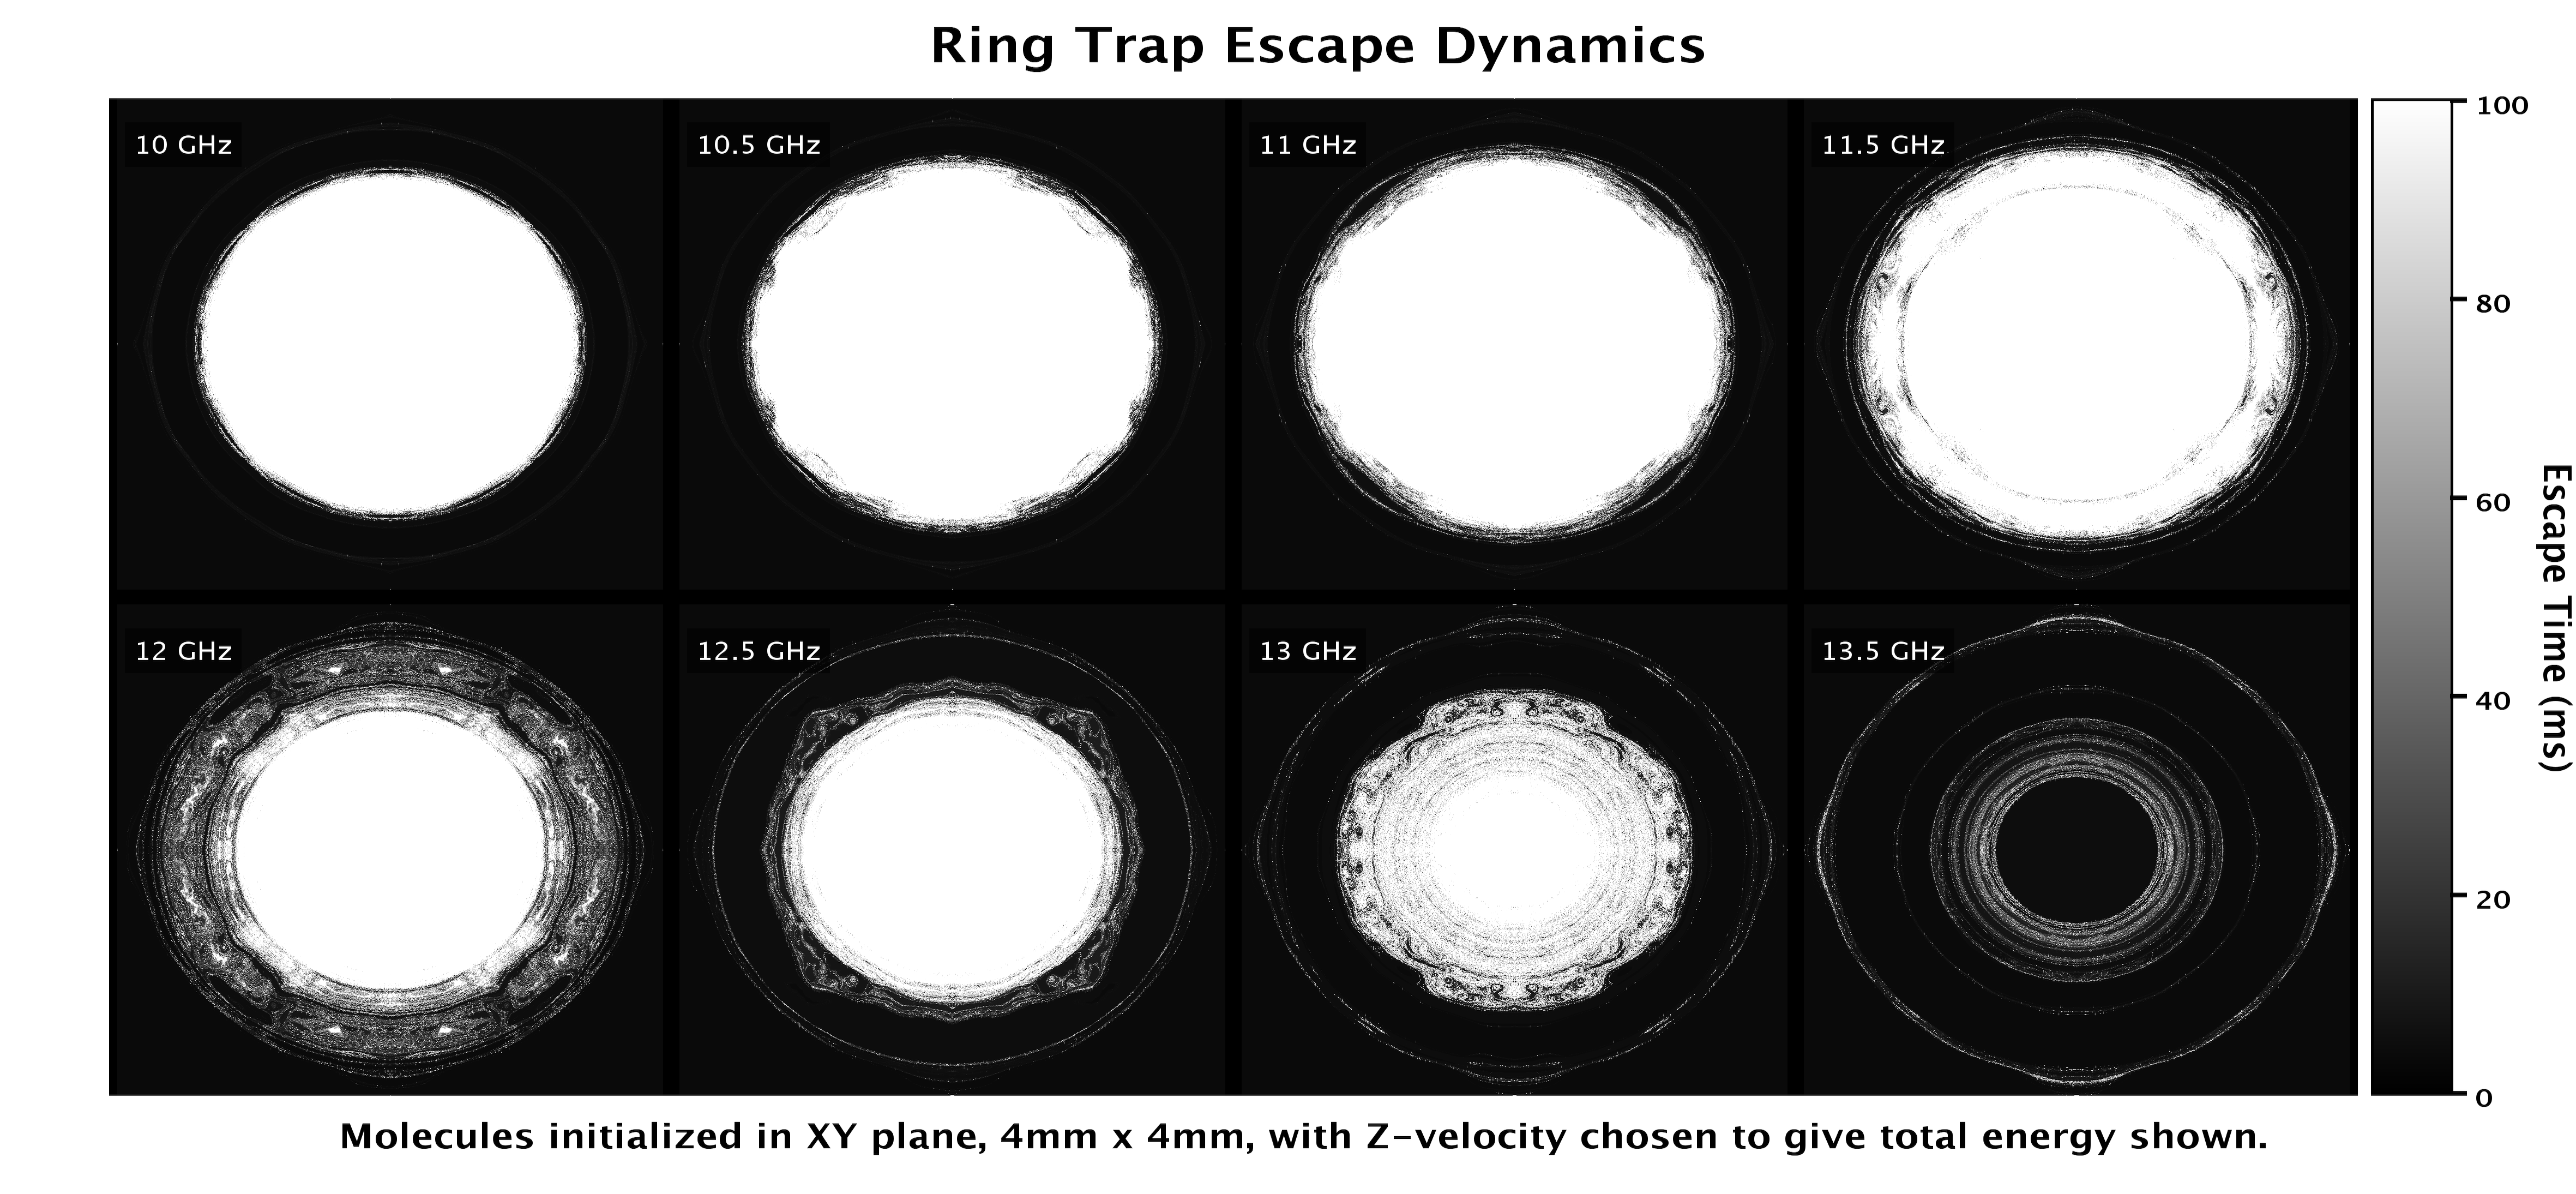
\includegraphics[width=13cm]{ringescape.png}\\
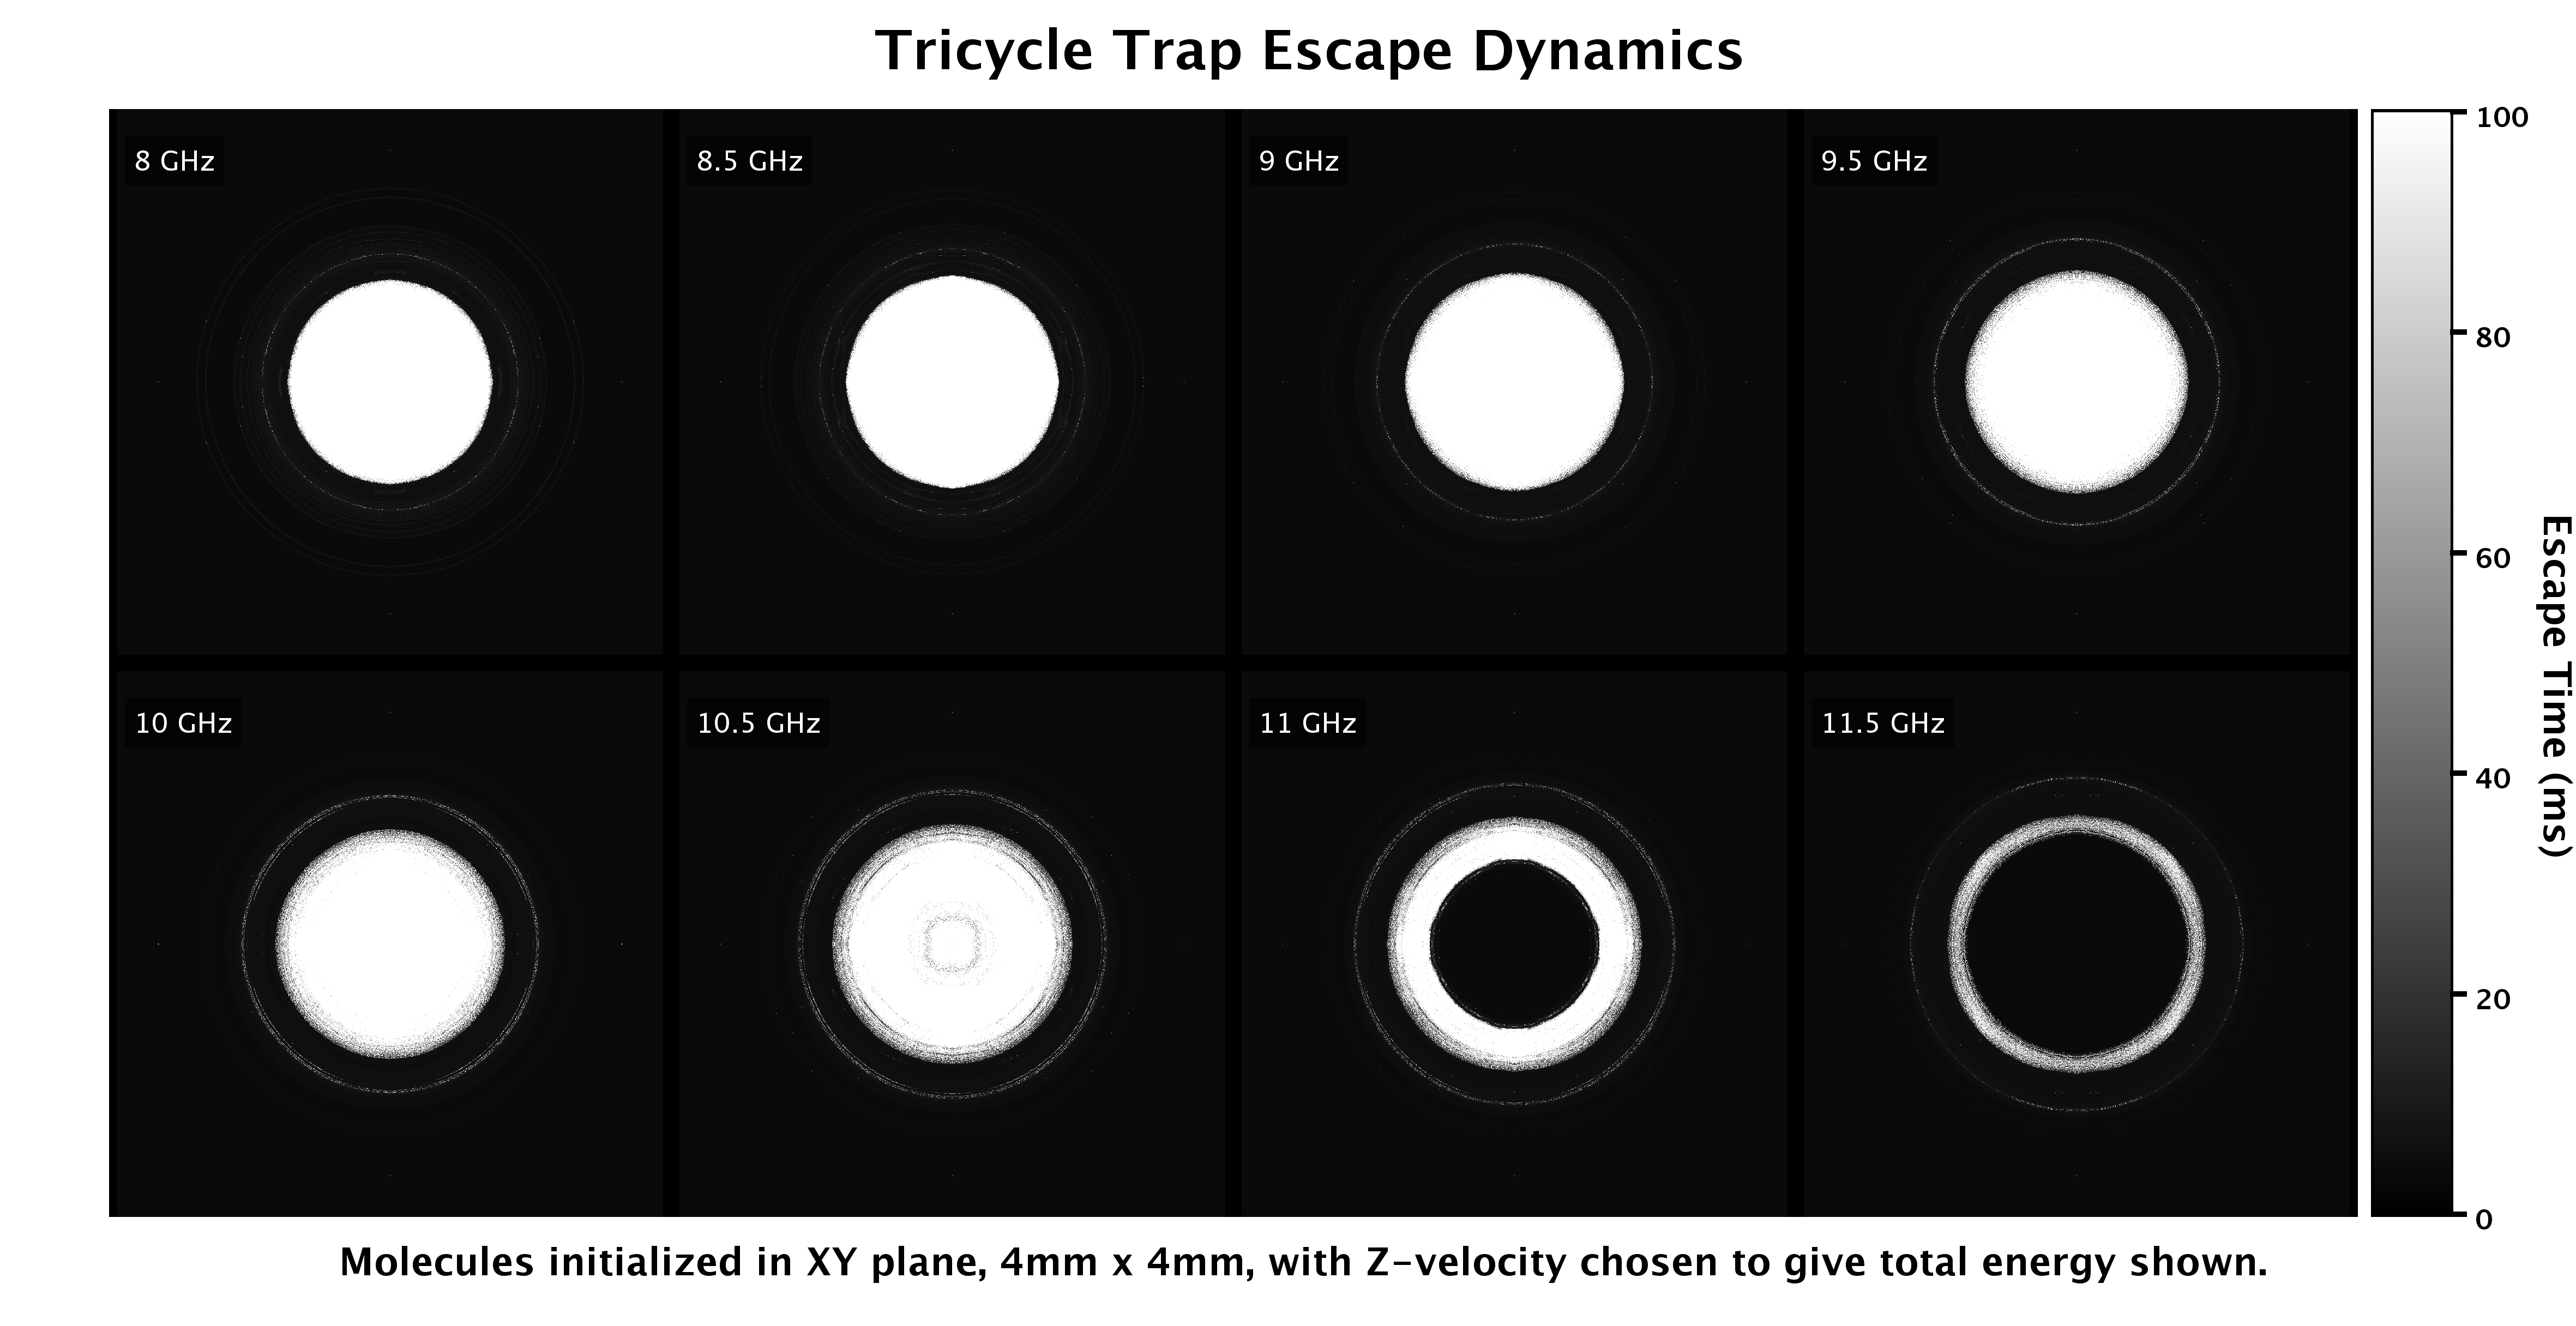
\includegraphics[width=13cm]{tricycleescape.png}\\
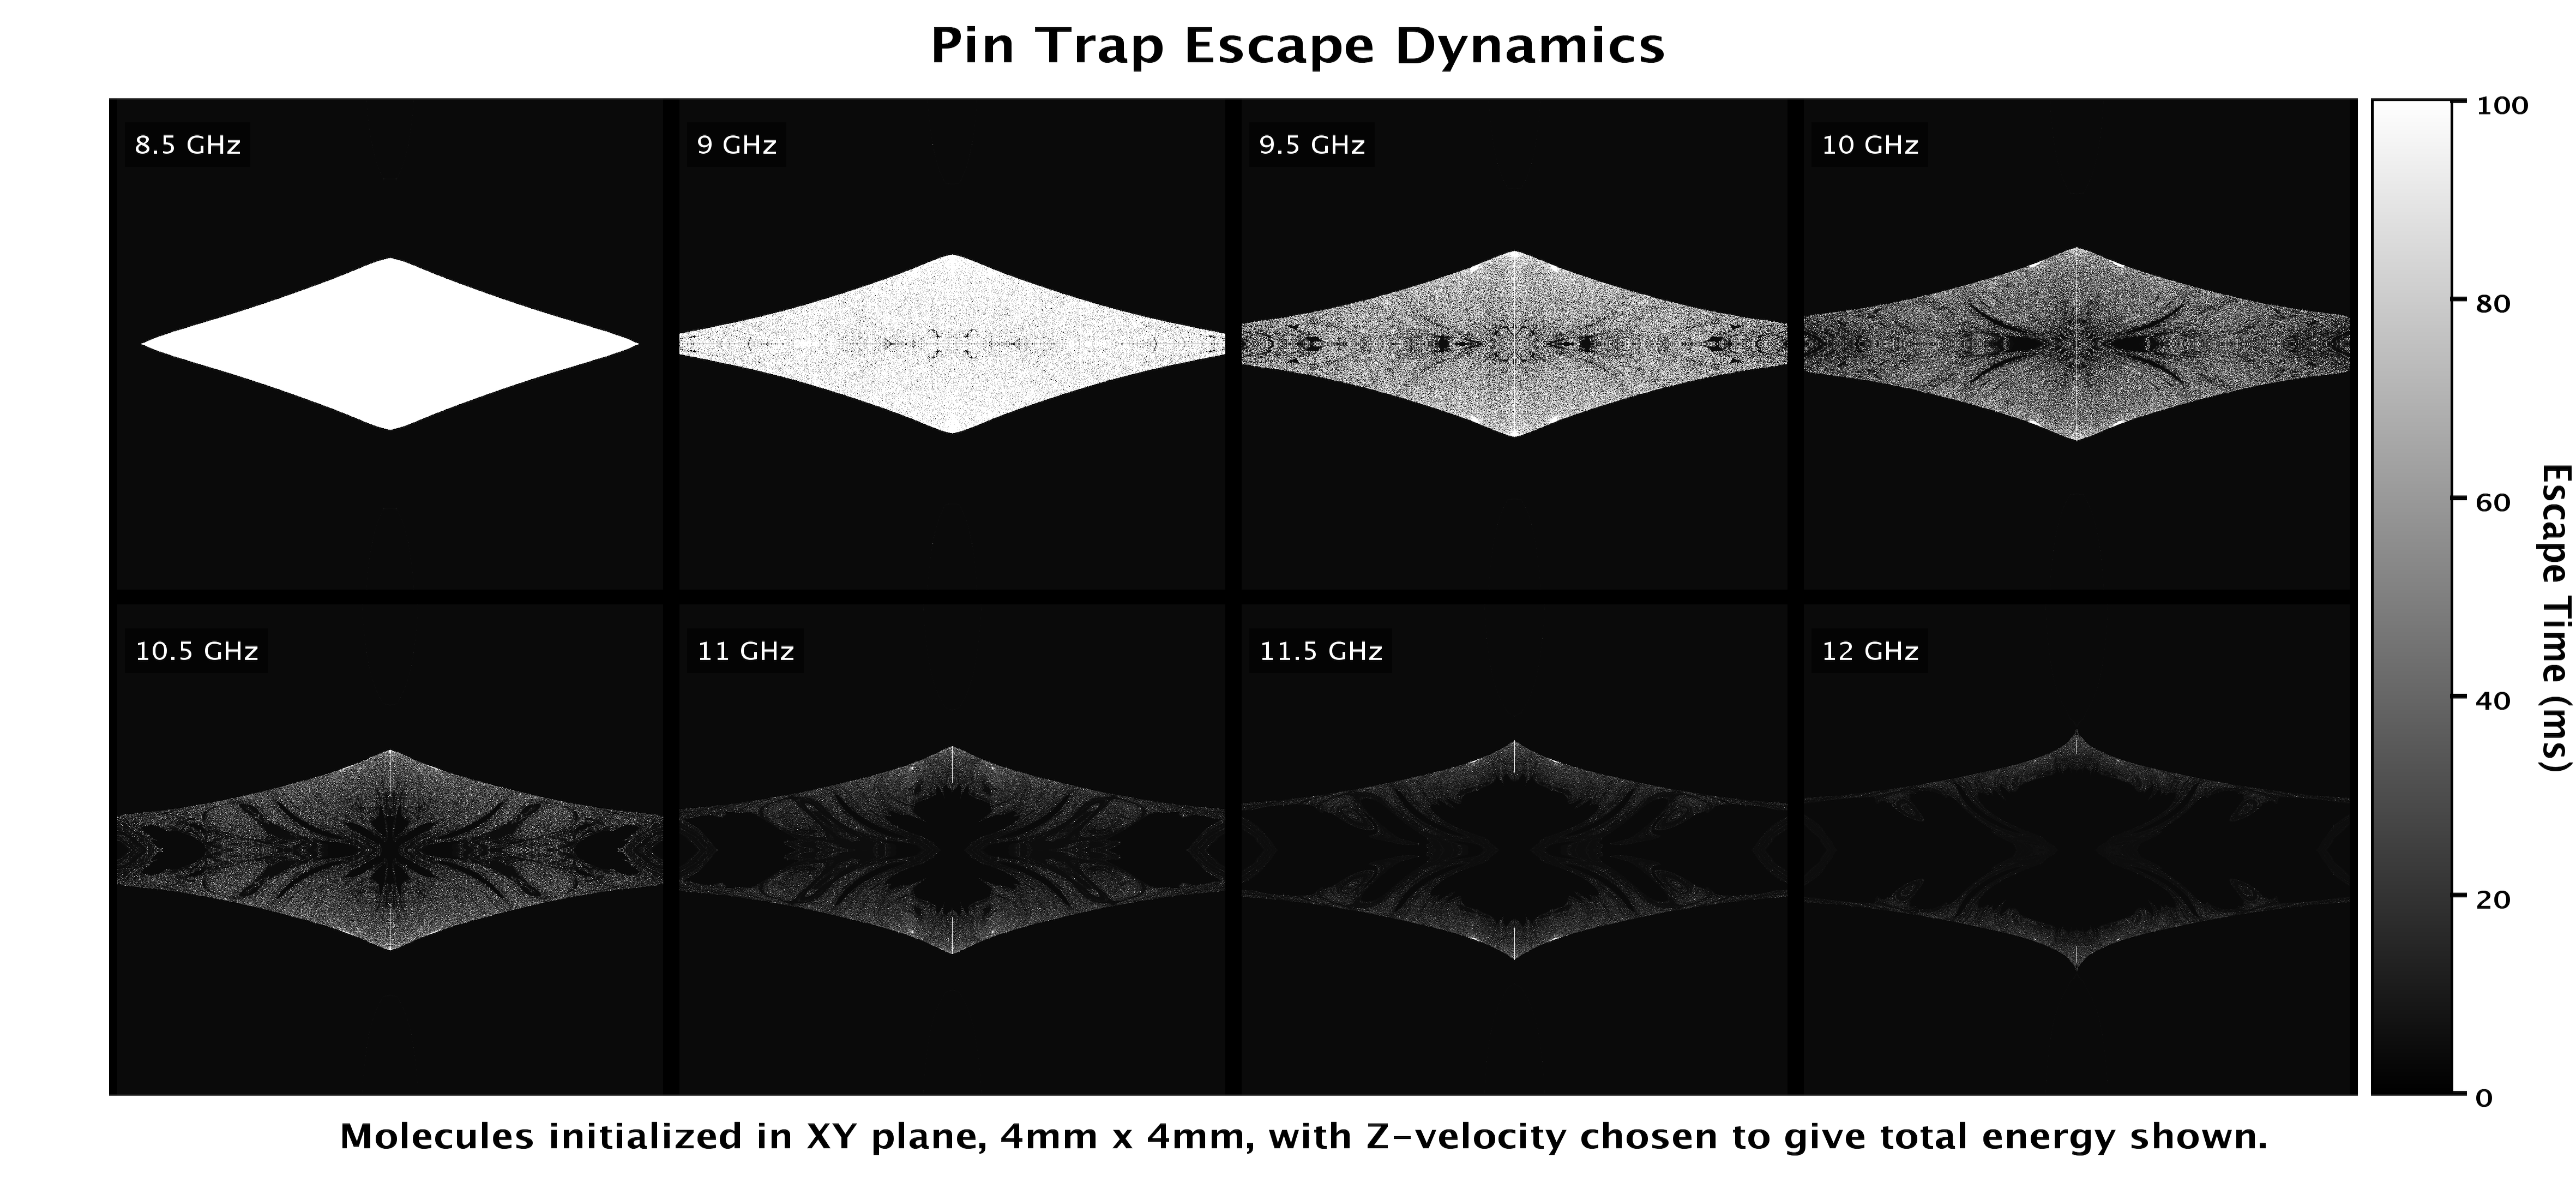
\includegraphics[width=13cm]{pinescape.png}
\caption[Escape Dynamics in the Ring, Tricycle and Pin traps.]{Molecules with the indicated total energy are initialized and their escape times indicated in grayscale. Position within a panel corresponds to initial position of the molecule in the transverse mid-plane of the trap.
\label{escapes}}
\end{figure}

I therefore followed this up by studying chaos indicators for trajectories in the magnetic pin trap.
This can be done by studying the evolution of orbits with infinitesimally varying initial conditions, in which case a new higher order equation of motion may be found which describes the evolution of the variation itself.
Specifically, if the evolution of the system is described by:
\begin{equation}
\frac{\partial x}{\partial t} = F(x,t),
\end{equation}
where $x$ is a point in 6D phase space and $F$ describes the ``flow'' of the system, then it is possible to specify a modification to the initial position $\delta x$ and study:
\begin{equation}
\frac{\partial x+\delta x}{\partial t} - \frac{\partial x}{\partial t}= F(x+\delta x,t) - F(x,t),
\end{equation}
which after making various leading order subtractions and so on gives rise to:
\begin{equation}
\frac{\partial \delta x}{\partial t} = \frac{\partial f}{\partial x}\cdot\delta x.  \label{eqvar}
\end{equation}

Various chaos indicators based on variational equations such as that in Eq.~\ref{eqvar} may be studied, such as the perhaps more well-known Maximum Lyapunov Exponent~\cite{wolf1985}.
Using a higher order variation called the $\text{OFLI}_2^{TT}$~\cite{Barrio2006}, I determined the pin trap to be a highly chaotic system, as the panels shown in Fig.~\ref{pinchaos} indicate.
A few stable orbits exist, but the majority are not.
It is also useful to verify that the software I developed for studying these indicators is in fact properly functioning.
In Fig.~\ref{chaosproof.png} I show how my results compare with those in~\cite{Gonzalez-Ferez2014}.
The comparison is nearly identical, which is especially remarkable given that I don't make use of the analytic expression for the crossed dipole trap~\citep[Eq.~6]{Gonzalez-Ferez2014}, since none is available for the magnetic pin trap.
Instead I use a spline to represent the potential.
This is described further in my publicly available code repository~\footnote{\href{https://github.com/dreens/ofli-OH-trapping}{Chaos Indicator Codebase}}.

\begin{figure}
\centering
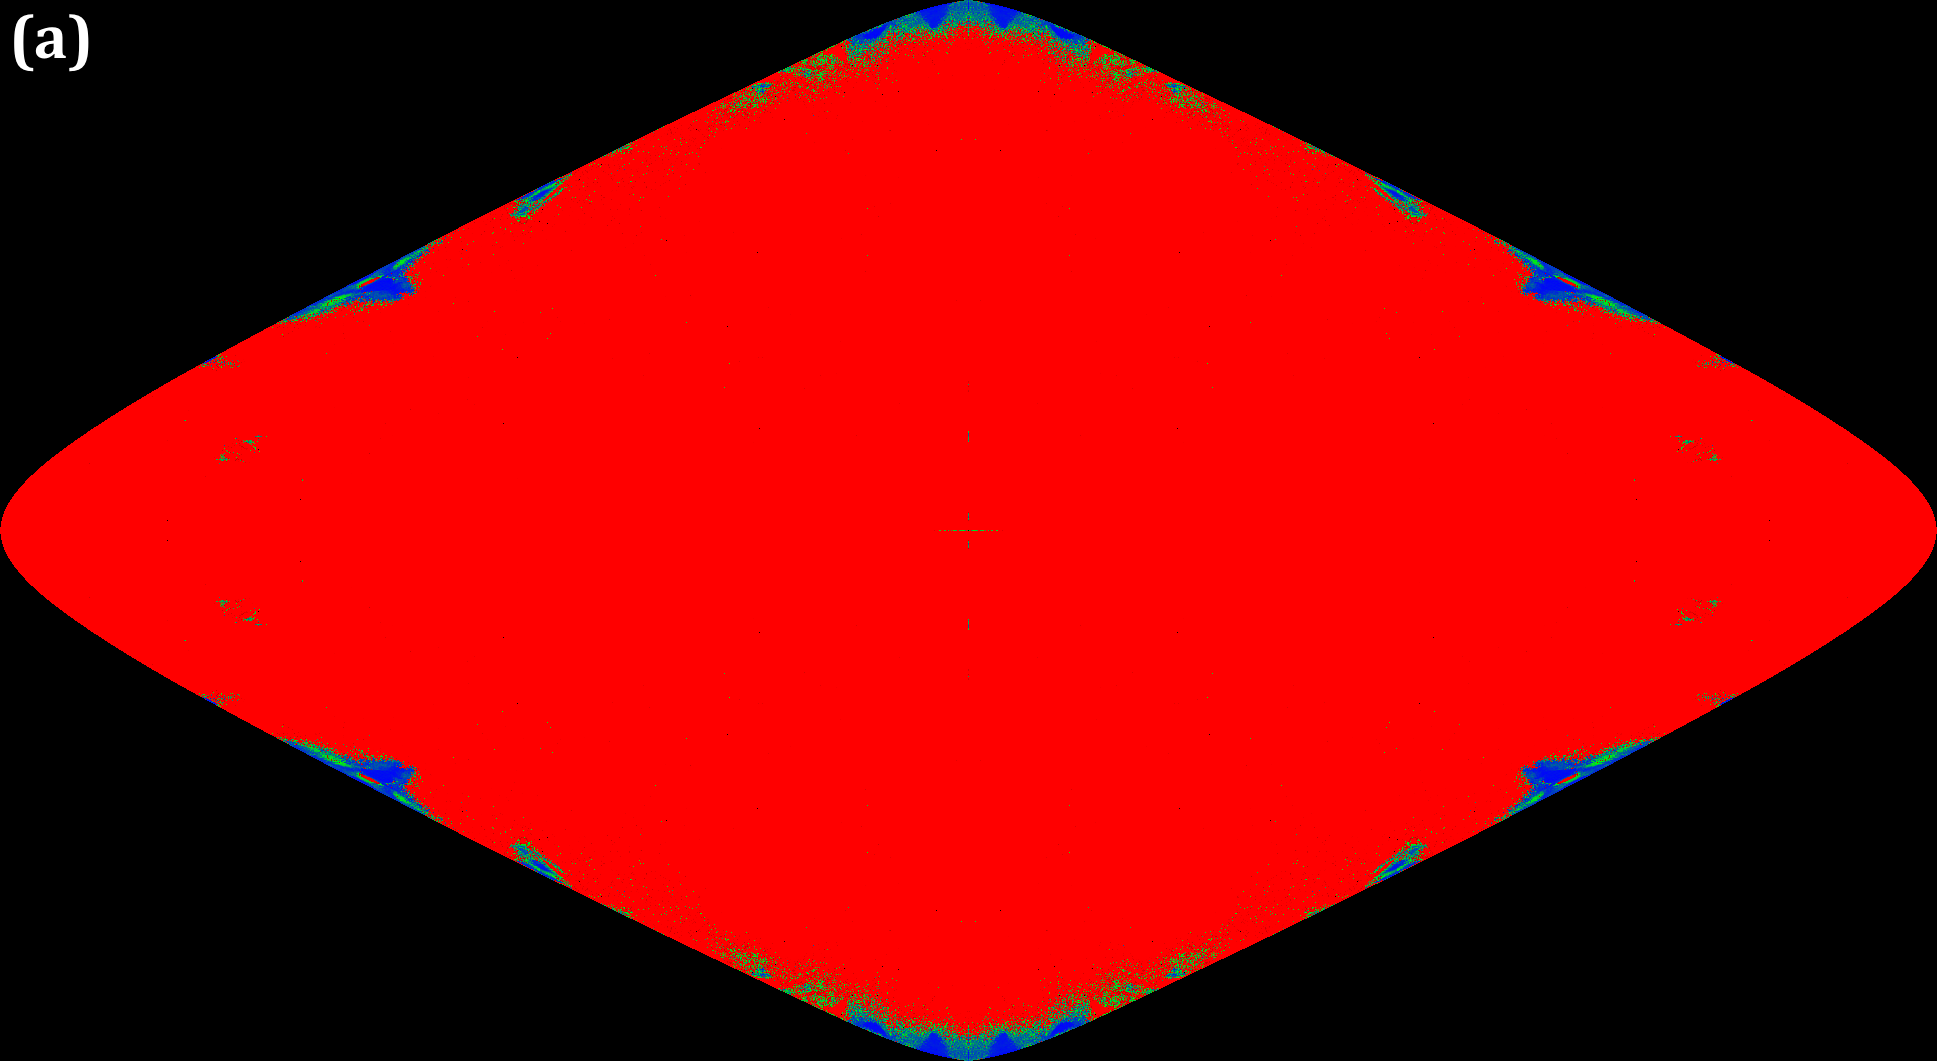
\includegraphics[width=11.4cm]{pin0p25xy.png}\hspace{4.5mm}
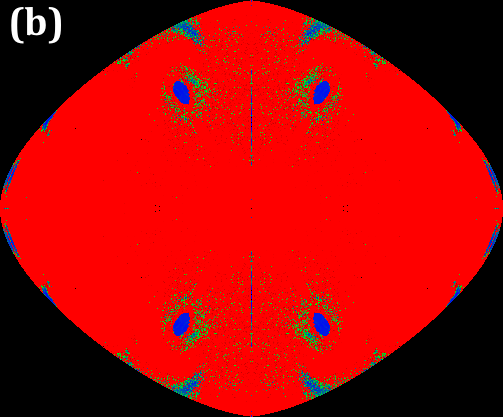
\includegraphics[width=3cm]{pin0p75xy.png}\\
\vspace{1mm}
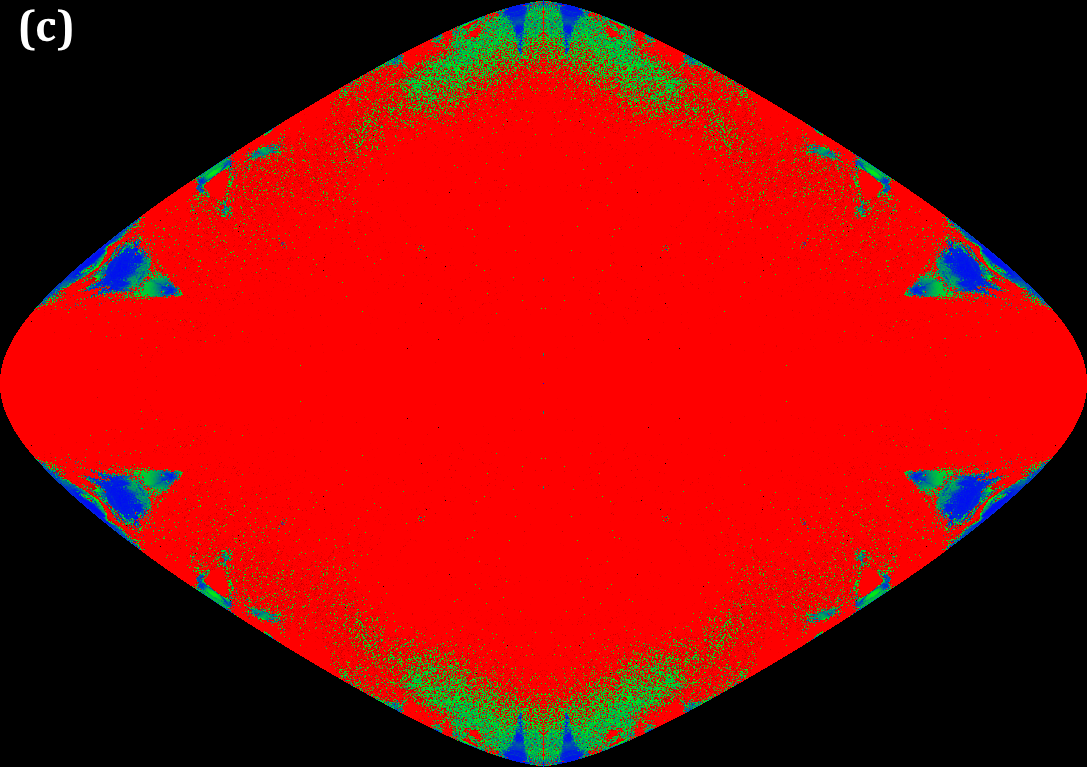
\includegraphics[width=6.5cm]{pin0p5xy.png}
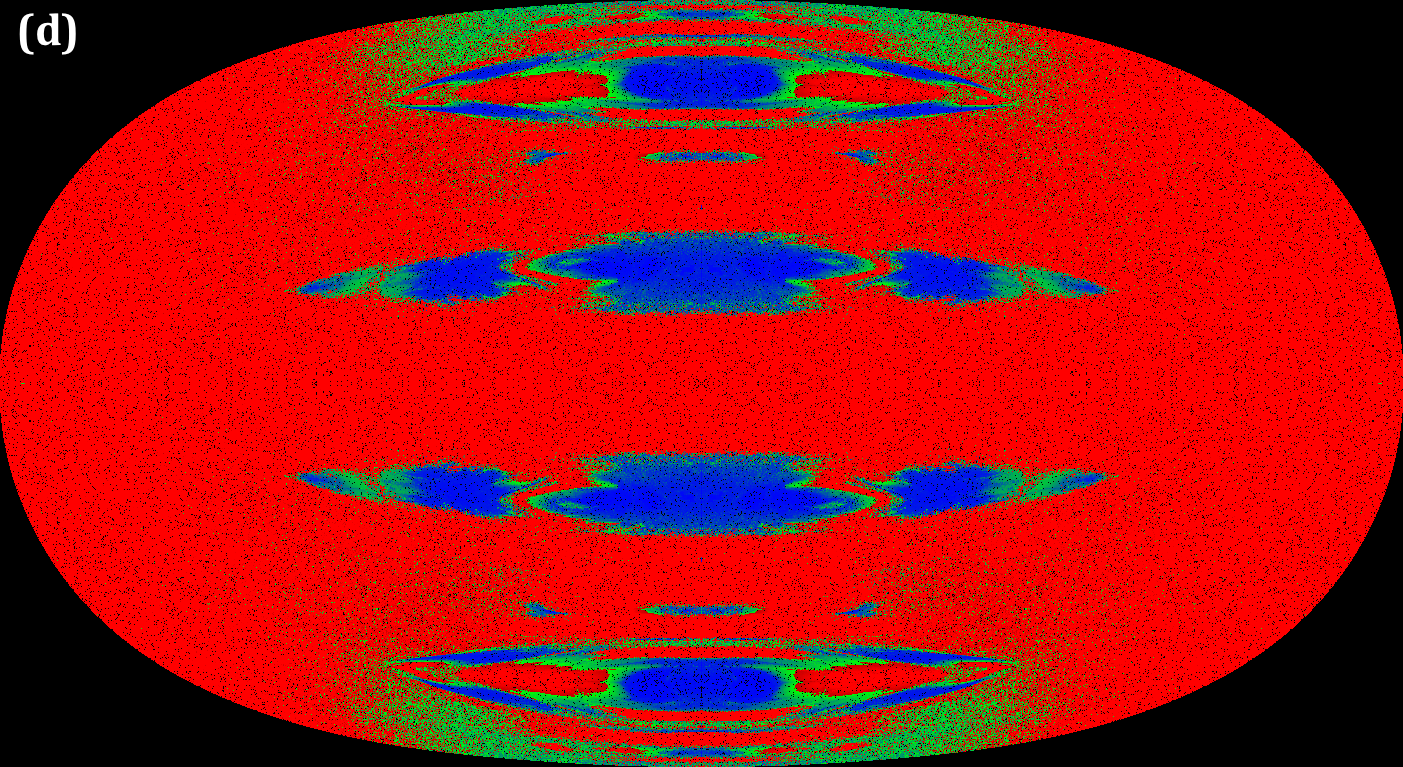
\includegraphics[width=8.4cm]{pin0p5yz.png}\\
%pin0p75xy.png
\caption[Chaos Indicators in the Pin Trap]{Chaos indicator $\text{OFLI}_{TT}^2$ is evaluated for trajectories beginning in the pin trap. Several islands of stability are engulfed within seas of chaos. Chaotic trajectories red, periodic blue, quasi-periodic green. The latter two vary on a color gradient. (a) $1.94$~mm wide, all panels to the same scale. Energies in this panel are $7.5$~GHz above trap minimum. Trajectories begin in the $x-y$ plane with velocity in the $z$ direction and normal to this plane. (b) $2.5$~GHz, $x-y$ plane. (c) $5$~GHz, $x-y$ plane. (d) $5$~GHz, $y-z$ plane. }
\label{pinchaos}
\end{figure}


\section{Next Generation Traps}

At the time of this writing, an effort is underway to develop a next generation magnetic trap suitable for use with our $333$ stage decelerator.
Thanks to the development of our engineering and manufacturing capabilities as far as cryogenics are concerned, I decided to push for a cryogenic trap.
This has the added benefit of addressing the vacuum and blackbody lifetime limits for OH molecules and potentially enabling ten second study times.
A number of features of this design are worth discussing here.

\subsection{Pin Trap Farewell}

We decided to move back to the 3D magnetic quadrupole design, despite the success of the magnetic pin trap for addressing spin flip losses.
Reasons for this include the following:
\begin{enumerate}
\item Difficulty in correctly selecting and orienting the magnetic pins, which required an in-vacuum translation stage and associated high voltage concerns. We also had to carefully scan the field of the pins to identify a well-matched pair.
\item Questions about the HV performance of the pins, which didn't condition very well. 
No major arcs during normal operation were occurring, but the loaded temperature was triple that predicted by sims, a possible indication of arcing type effects during loading.
\item Maintaining the Bias coil, which required a high pressure water boosting system~\cite{Reens2017booster}
\item Expectations about collisional behavior. The pin trap resolves spin-flip losses, but substates nonetheless come quite close to one another over a broad spatial range, making inelastic loss probable. At one point Goulven Qu\'em\'ener actually calculated inelastic cross sections for a map of fields and angles in the pin trap and confirmed this.
\item Lifetime concerns for the magnetic pins themselves. We had a number of pins demagnetize during conditioning, leading us to install an in-vacuum temperature probe which could be made to touch the pins using a manipulator feedthrough or brought safely away from them during the application of voltage.
\end{enumerate}

\subsection{Magnets}

Neodymium magnets reversibly demagnetize to $70\%$ of their room temperature strength when brought to temperatures in the $10$~K regime, but newer Praseodymium magnets actually enhance~\cite{Shea2010}.
I was able to coordinate the manufacture of these for our application\footnote{\href{https://www.vacuumschmelze.com}{Vacuumschmelze} manufactures these and has a US distribution team based in Kentucky. Thanks to Ed Narevicius for the referral. Grade 131 TP and 131 DTP.}.

An effort was undertaken to more systematically study the variation of the performance of the system as far as various dimensions are concerned.
A tricycle style was selected, though with a bit of a reduction in gradient.
Radiusing the rear electrode was considered, as well as variations in the thickness of extra surfaces designed to cover the imperfect surfaces of the magnets.
In all cases, deceleration and loading dynamics were included, with the exception of \fm3 effects.
I have only once made an attempt at including these effects, for the sake of more precisely fitting the escape dynamics of molecules in the tricycle trap with extra electric field turn-on events, described further in Chap.~\ref{chapter:collisions}.
The final selected geometry is shown in Fig.~\ref{cryocycle.png}, and is dubbed the Cryocycle.

\figdave{cryocycle.png}{Cryocycle Field Distributions}{Relevant information for the Cryocycle trap under manufacture at the time of this writing. (a) Magnetic field magnitude, $500$~G per contour, trap depth of $\sim2200$~G transversely. (b) Electric field magnitude during loading. $10$~kV/cm per contour. Curved rear surface acts to extend the region of steep trapping slope further towards the rear magnet relative to the Tricycle trap, see Fig.~\ref{NearFieldUWave.png}a. (c) Raytrace performed in COMSOL Multiphysics for determining collection solid angle close to $4$~sr for the Cryocycle.}{\linewidth}

\subsection{Photon Collection}

The cryocycle also features what will hopefully serve as an important improvement in fluorescence collection.
Mounted together with the magnet is an elliptical reflector capable of directing much of the fluorescence from the trapped molecules onto a PMT outside the vacuum.
Collection solid angles close to $4$~sr should be possible, an order of magnitude improvement over the previous traps, see Fig.~\ref{cryocycle.png}c.
Of course this assumes a highly reflective surface, only obtainable in the near ultraviolet with Aluminum~\cite{rumble2017crc}, which is fortunately a good choice for thermal conductivity as well.
Aluminum may be a less ideal choice as far as high voltage is concerned however, since its surface oxide layer should enable the formation of patch charges and stray electric fields to some extent.
This could prove especially problematic in the event of any sensitive long-term studies, since variations in the patch charges could lead to variations in the enhancement of spin-flip losses near the trap center.
One technique to address this is to detect the magnitude of spectroscopy, see Fig.~\ref{strayhyperspec.png}.
Because of the small magnitude of the differential Zeeman shift, slight perturbations of the electric fields on the magnetic field dependent lineshapes, especially in the vicinity of avoided crossings, are clearly discernable.
Performing a full spectroscopic sequence would be slow, but similar observables could be designed to give sensitivity to stray electric fields, for example a two-point spectroscopy comparing the frequency of the dip to that of the peak.
Another possibility would be to look for population transfer at a more distant frequency that would only address molecules close to avoided crossings.

\figdave{strayhyperspec.png}{Stray Field Influences Spectroscopy}{Stray fields are seen to influence spectroscopy. 
The black simulated line corresponds to $10$~V/cm. 
The two dips correspond to the inability of microwaves to address molecules at those frequencies due to avoided crossings perturbing the lines at those locations. 
Only one crossing is significantly perturbed by small fields, that between \e3 and \f1, but this crossing occurs in two different locations for the two nuclear spin substates of \f3.}{\linewidth}

\subsection{Blackbody Absorption}

In order to benefit from a lifetime extension with cryogenic temperatures, it is necessary to carefully control the radiation environment of the molecules. OH can absorb radiation primarily at $120~\mu$m ($2.5$~THz)~\cite{Hoekstra2007}, where typical radiation shielding conductors have near perfect reflection.
In the case of an incomplete shield, as is required for our setup since the shield cannot approach to close to the high voltage decelerator, this can mean that the radiation relevant for the molecules is actually fully equilibrated to room temperature despite the cryogenic shield.
Whatever the dominant absorbers are for the relevant wavelength will dominate the radiation environment, with conductive surfaces playing little to no role.
Many materials are surprisingly transparent, including plastics such as Teflon which are actually used as lenses~\footnote{\href{https://www.thorlabs.com/newgrouppage9.cfm?objectgroup_id=1627}{Teflon Lenses}}.
To address this, I opted for the addition of ceramic plates on the inside of our radiation shield to influence the radiation environment by absorbing THz radiation otherwise reflected by the shields.

\subsection{Cloverleaf Trapping}

Of course it would be ideal to address the issue of electric field enhanced loss once and for all with a lifted magnetic trap.
This is possible with permanent magnets, and a streamlined design was identified and simulated, see Fig.~\ref{cloverleaf.png}.
Such a trap may one day be the right choice, but it would seem unwise to tackle this simultaneously with the changes already being introduced.
Moreover, without collisional effects, it may not be worth the effort.
These effects should be more clearly evidenced in the Cryocycle, which should feature at least an order of magnitude improvement over any cloverleaf style design in the densities which may be loaded.
The reason for this is that cloverleaf type geometries always require a delicate competition between the strengths of different fields, and can never be generated with the same trap depths or gradients as the quadrupole trap.
The design shown in Fig.~\ref{cloverleaf.png} loads only $20\%$ of the Cryocycle, and is significantly less tight, likely at least twofold reduction in each direction, for a forty-fold reduction in density relative to the Cryocycle.

\figdave{cloverleaf.png}{Permanent Magnetic Cloverleaf Trap}{
(a) Earlier Design from Matt Hummon, $32$ one eighth arc segments. 
(b) Updated design, $8$ quarter arc segments, $2$ rings, $1$ disk. $4$~mm gap between magnets.
(c) Magnetic Trap. Much longer than wide, unlike 3D quadrupole traps. Up to $1200$~G deep or so, depending on tuning of extra disk magnet. 
(d) Loading fields, much less ideal than Tricycle trap, concave up across trap center and steepest out front.}{\linewidth}

If at some point it becomes necessary to pursue the Cloverleaf trap in earnest, a few points are worth mentioning.
Firstly, always make sure to investigate cross sections through the trap in many planes, since often the three principal orthogonal planes can miss the actual weak points of the trap.
It should be sufficient to add in planes with $\theta=\pi/4$ and including the $z$ axis, working in cylindrical coordinates, for the Cloverleaf shown in Fig.~\ref{cloverleaf.png}b, but for that in Fig.~\ref{cloverleaf.png}a, I believe the weak points may occur in the $\theta=\pi/8$ planes.
Secondly, for any given geometry it is always worth varying the magnitude of an extra bias magnetic field in the z direction before making conclusions.
This extra field can have a very significant effect on the tightness and depth of the trap, and in practice may even be tuned in the experiment with an external coil or a translatable permanent magnet.
I had some success with removing a small divot from the rear electrode so as to reduce loss of molecules which can access that volume.
It helps the loading significantly to add conductor between the magnets and touching the front magnets closest to the decelerator, so as to push the loading hill further back and overlap the trap center better.
One problem with this is that then the collection solid angle is negatively impacted.
Mounting the magnets in aluminum frames that are highly polished to better allow fluorescence to escape could help with this, as planned in the Cryocycle.
Finally, it will be important to study this trap outside of the the vacuum somehow, especially in order to see how closely the magnets can be packed/glued together, what the resulting field strengths are, and especially to make sure that the trap is truly plugged.
This will require a highly miniaturized magnetic field probe of some kind.

\section{Trapping of Water Isotopologues}

One potentially exciting capability of our new lengthier decelerator system and advanced field distributions would be to apply it to a less Stark responsive molecule such as water~\citep[Sec.~2.4]{VanDeMeerakker2006thesis}.
The precise feasibility depends on just how slow the beam is when produced in Xenon in an Even-Lavie valve, which may be worth investigating in the near term.
An electrostatic quadrupole trap would be most feasible, and this could be achieved in a very similar system to the one currently planned for the Cryocycle, but with magnet-less electrodes.
The final pins of the decelerator can form one electrode of the quadrupole, which would then require an additional ring and endcap electrode.
Detection could be performed with some sort of REMPI scheme, but for initial tests of decelerability the RGA may suffice.

\bibliographystyle{unsrtDR}	% or "siam", or "alpha", etc.
\bibliography{allrefs}		% Bib database in "allrefs.bib"
\end{document}




